\section{Advantages of Versatile Policies and Source of Robustness}\label{sec:multi_skill}


\begin{figure*}[t]
\centering
\begin{subfigure}{0.487\linewidth}
  \centering
  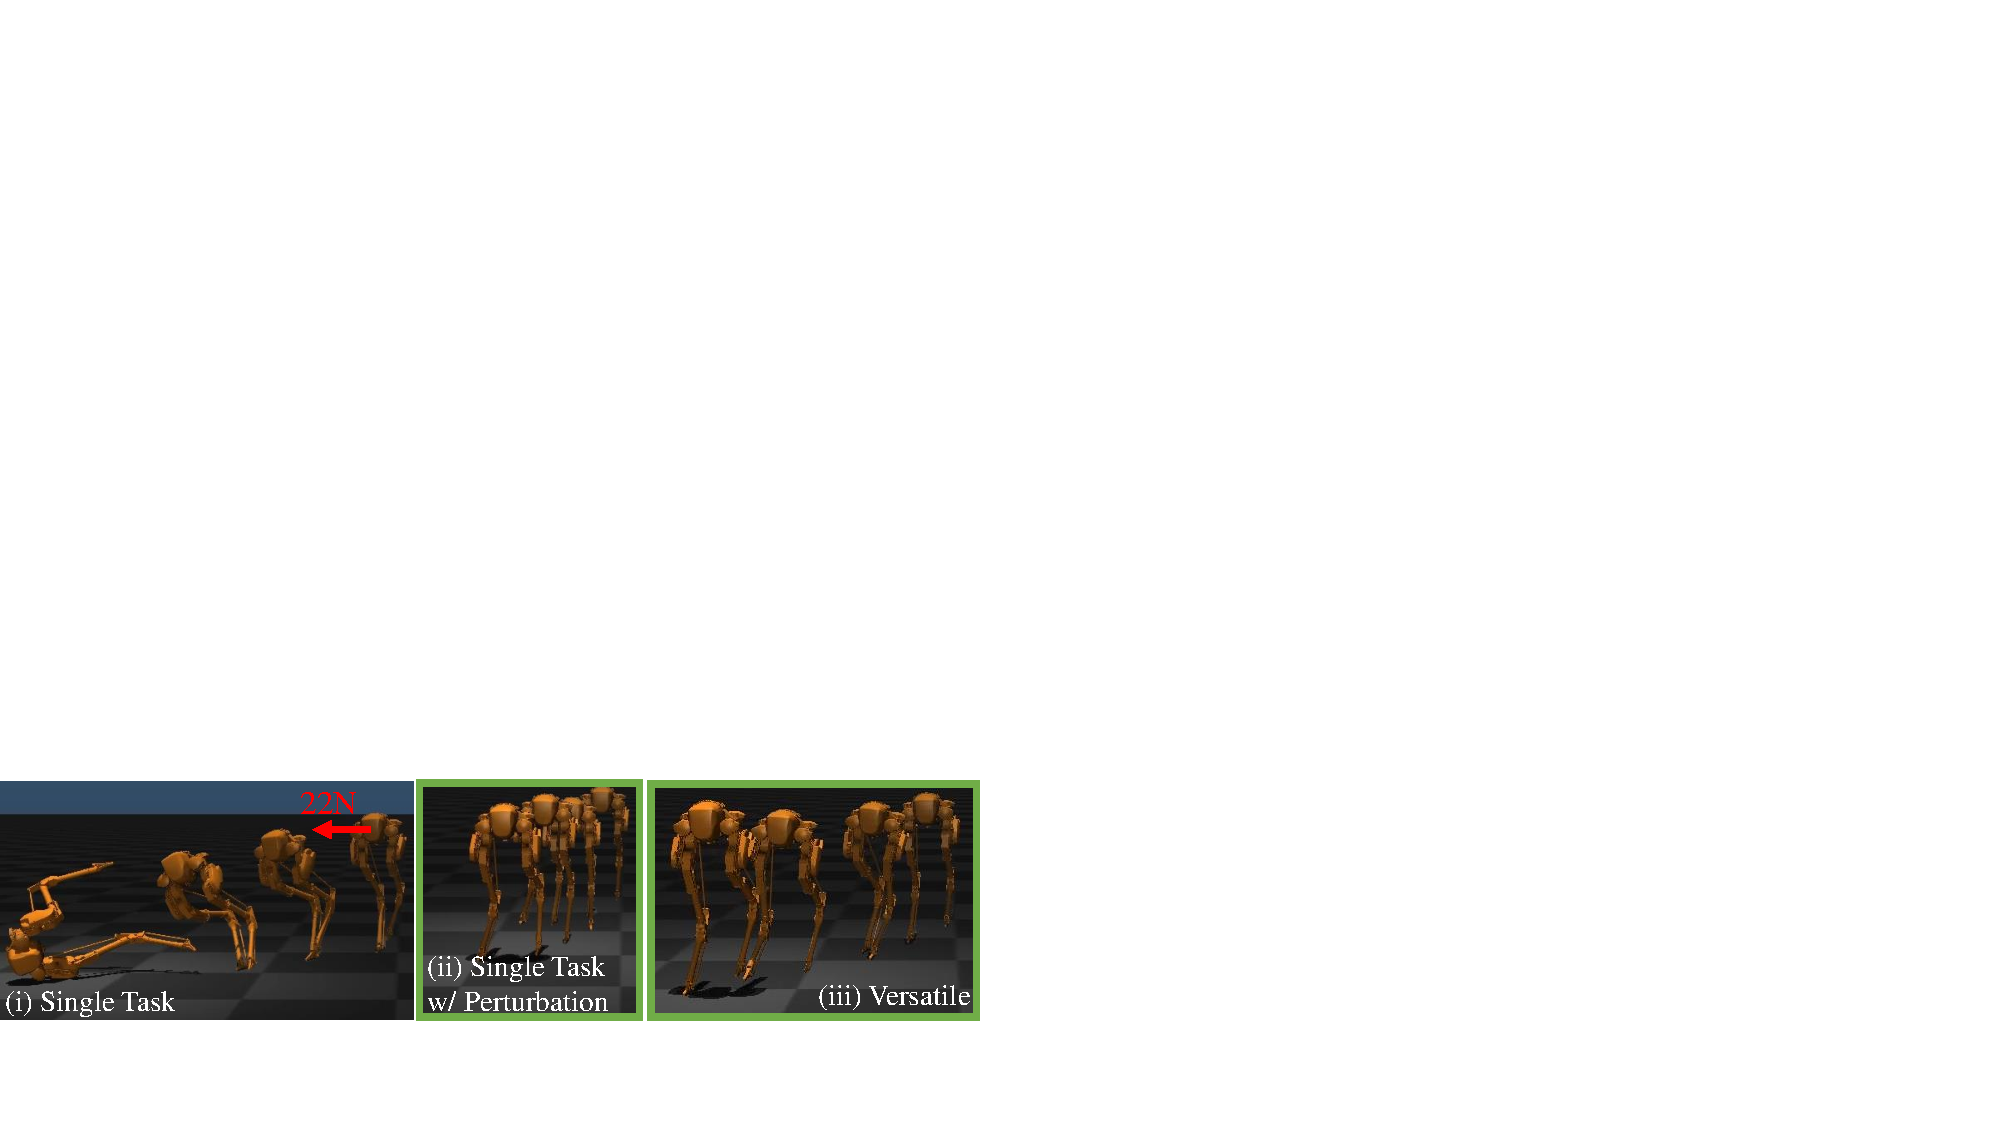
\includegraphics[width=\linewidth]{figures/bm_walk_perturb.pdf}
  \caption{Walking with Consistent Unknown Lateral Perturbation Force}
  \label{subfig:bm_single_sim_perturb_walk}
\end{subfigure}
\begin{subfigure}{0.5\linewidth}
  \centering
  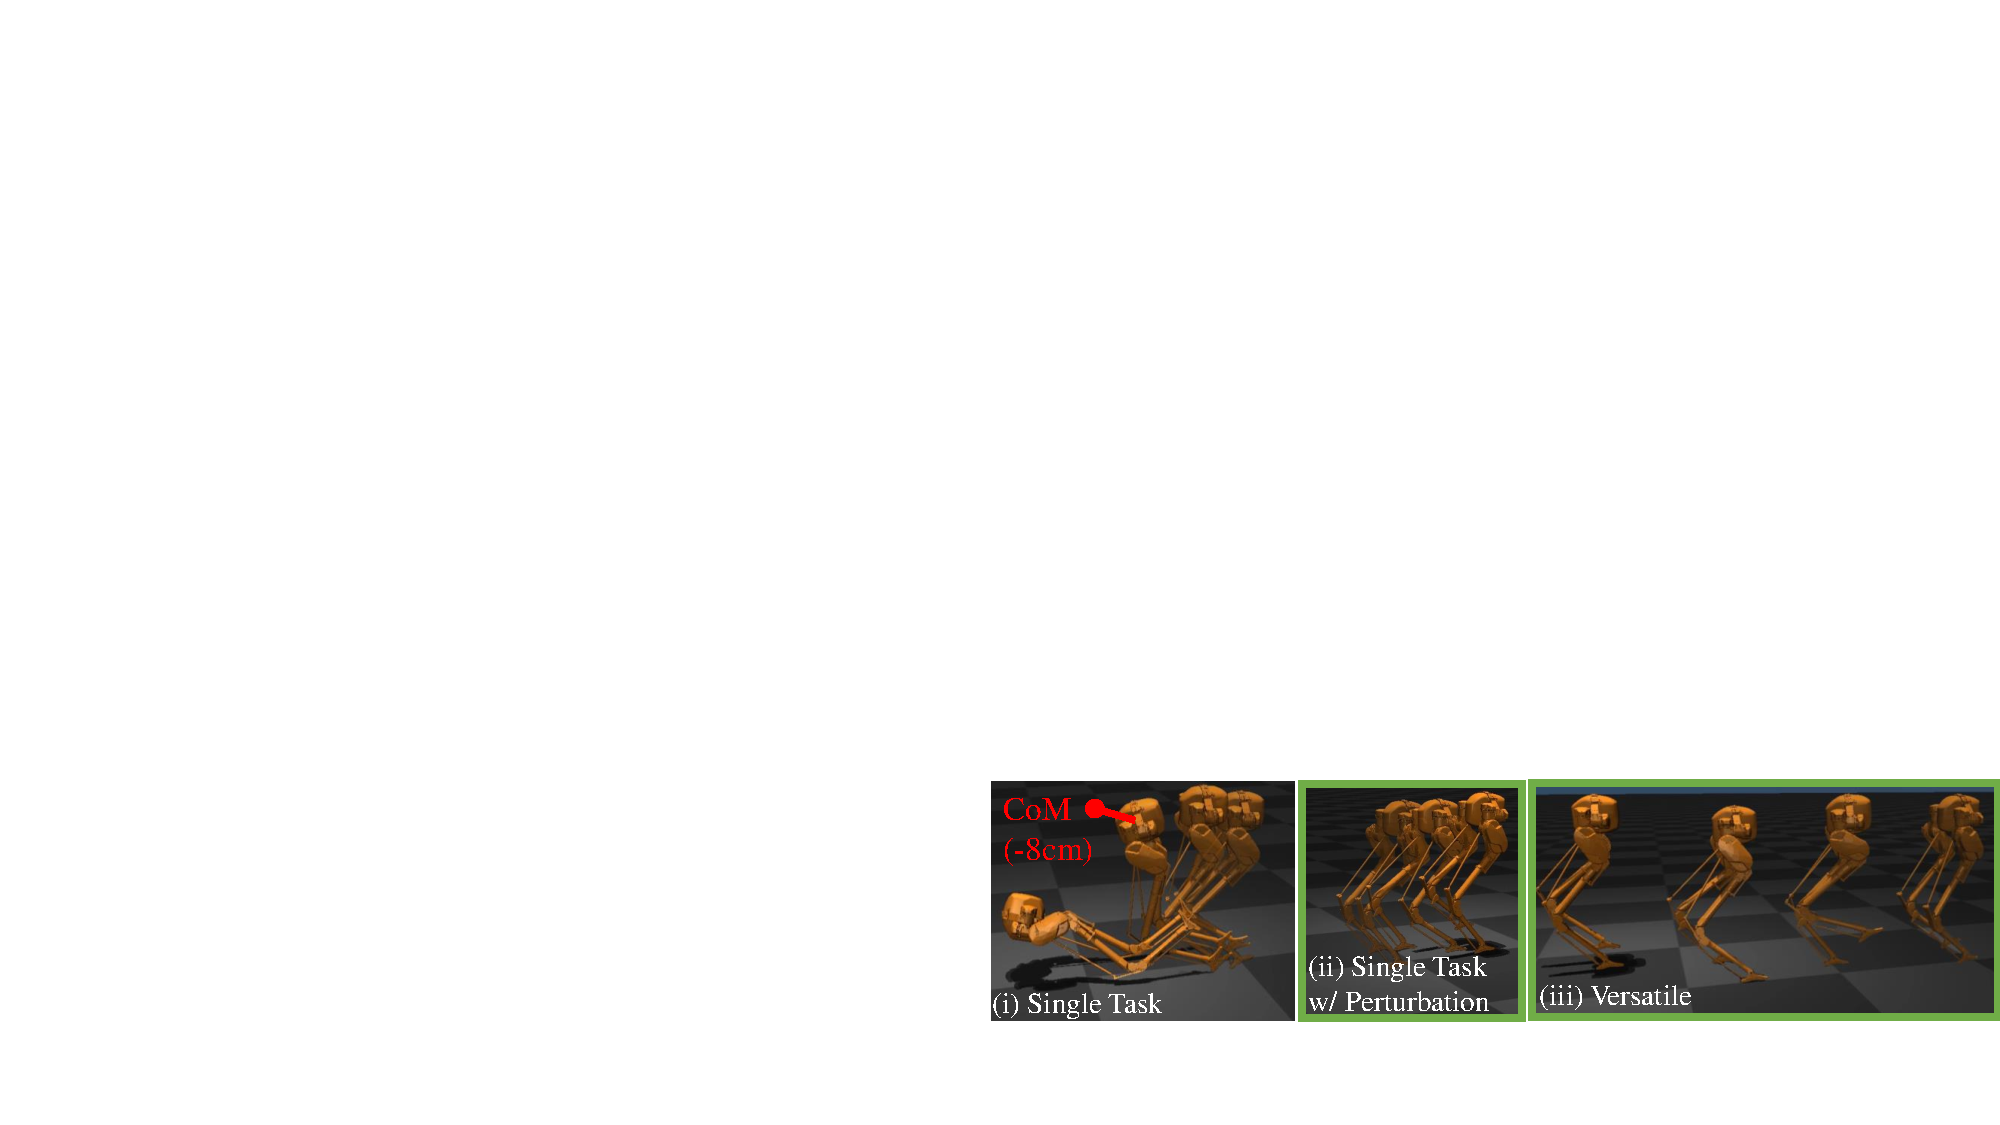
\includegraphics[width=\linewidth]{figures/bm_walk_ipos.pdf}
  \caption{Walking with Errors in Center of Mass Positions of All Links}
  \label{subfig:bm_single_sim_ipos_walk}
\end{subfigure}
\begin{subfigure}{\linewidth}
  \centering
  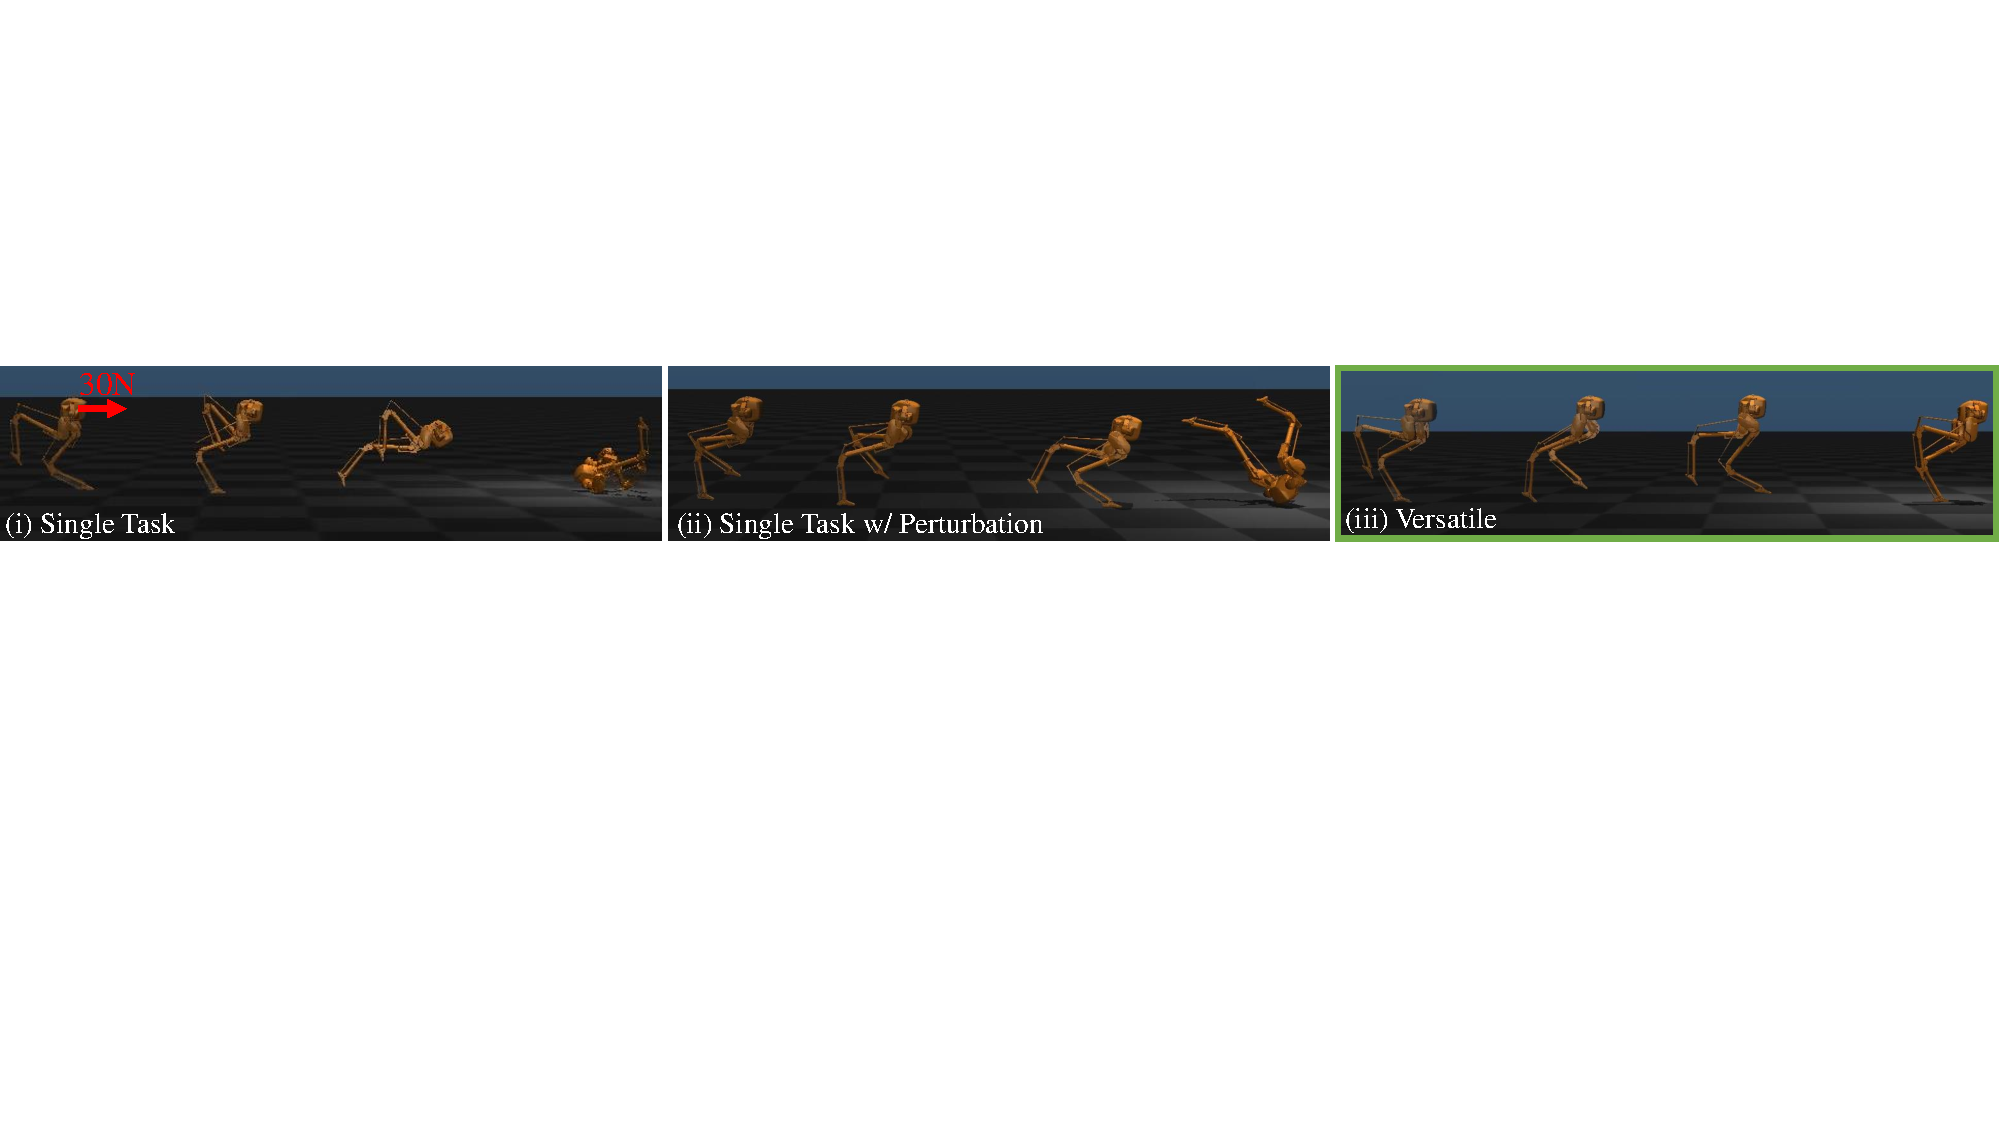
\includegraphics[width=\linewidth]{figures/bm_run_perturb.pdf}
  \caption{Running with Consistent Unknown Lateral Perturbation Force}
  \label{subfig:bm_single_sim_perturb_run}
\end{subfigure}
\begin{subfigure}{\linewidth}
  \centering
  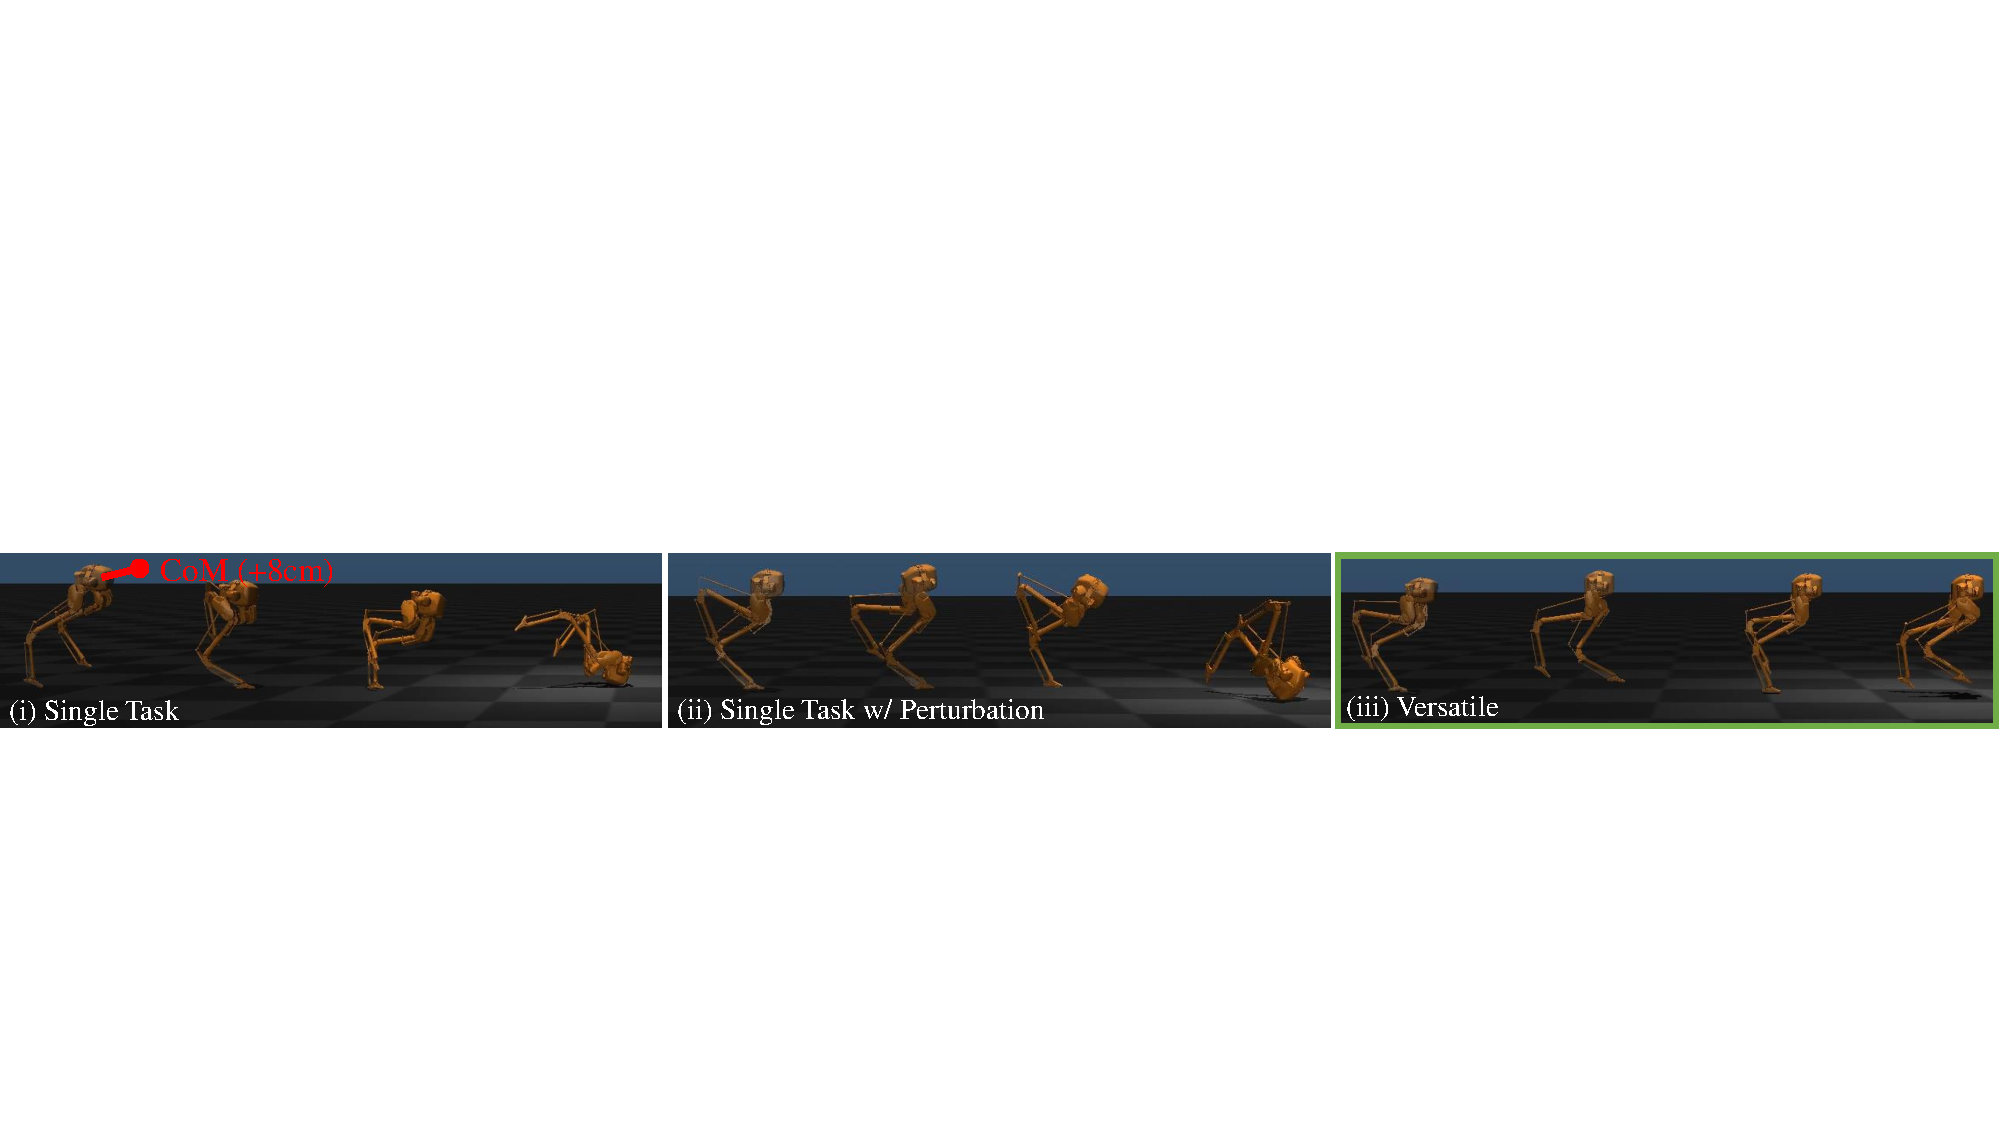
\includegraphics[width=\linewidth]{figures/bm_run_ipos.pdf}
  \caption{Running with Errors in Center of Mass Positions of All Links}
  \label{subfig:bm_single_sim_ipos_run}
\end{subfigure}
\begin{subfigure}{0.4425\linewidth}
  \centering
  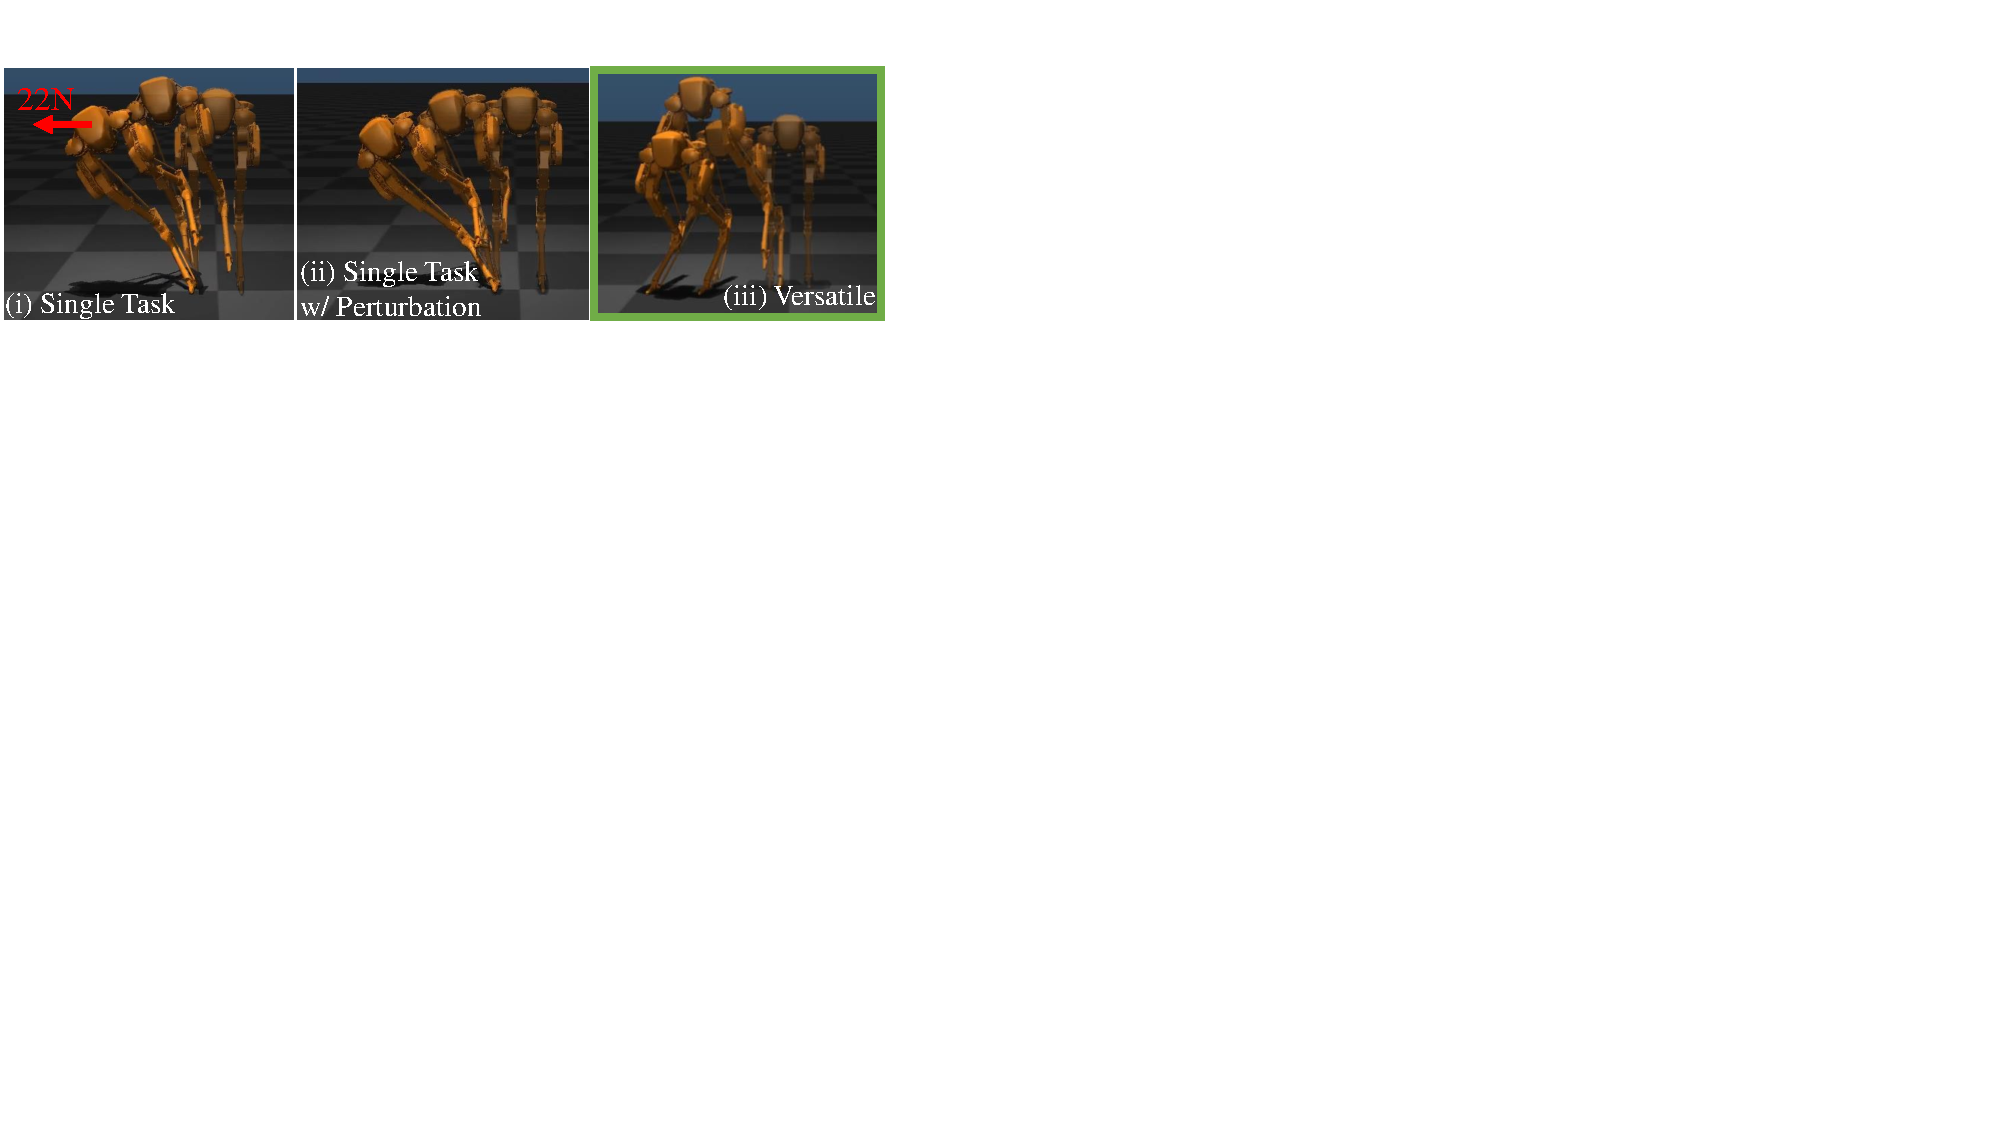
\includegraphics[width=\linewidth]{figures/bm_jump_perturb.pdf}
  \caption{Jumping with Consistent Unknown Lateral Perturbation Force}
  \label{subfig:bm_single_sim_perturb_jump}
\end{subfigure}
\begin{subfigure}{0.5425\linewidth}
  \centering
  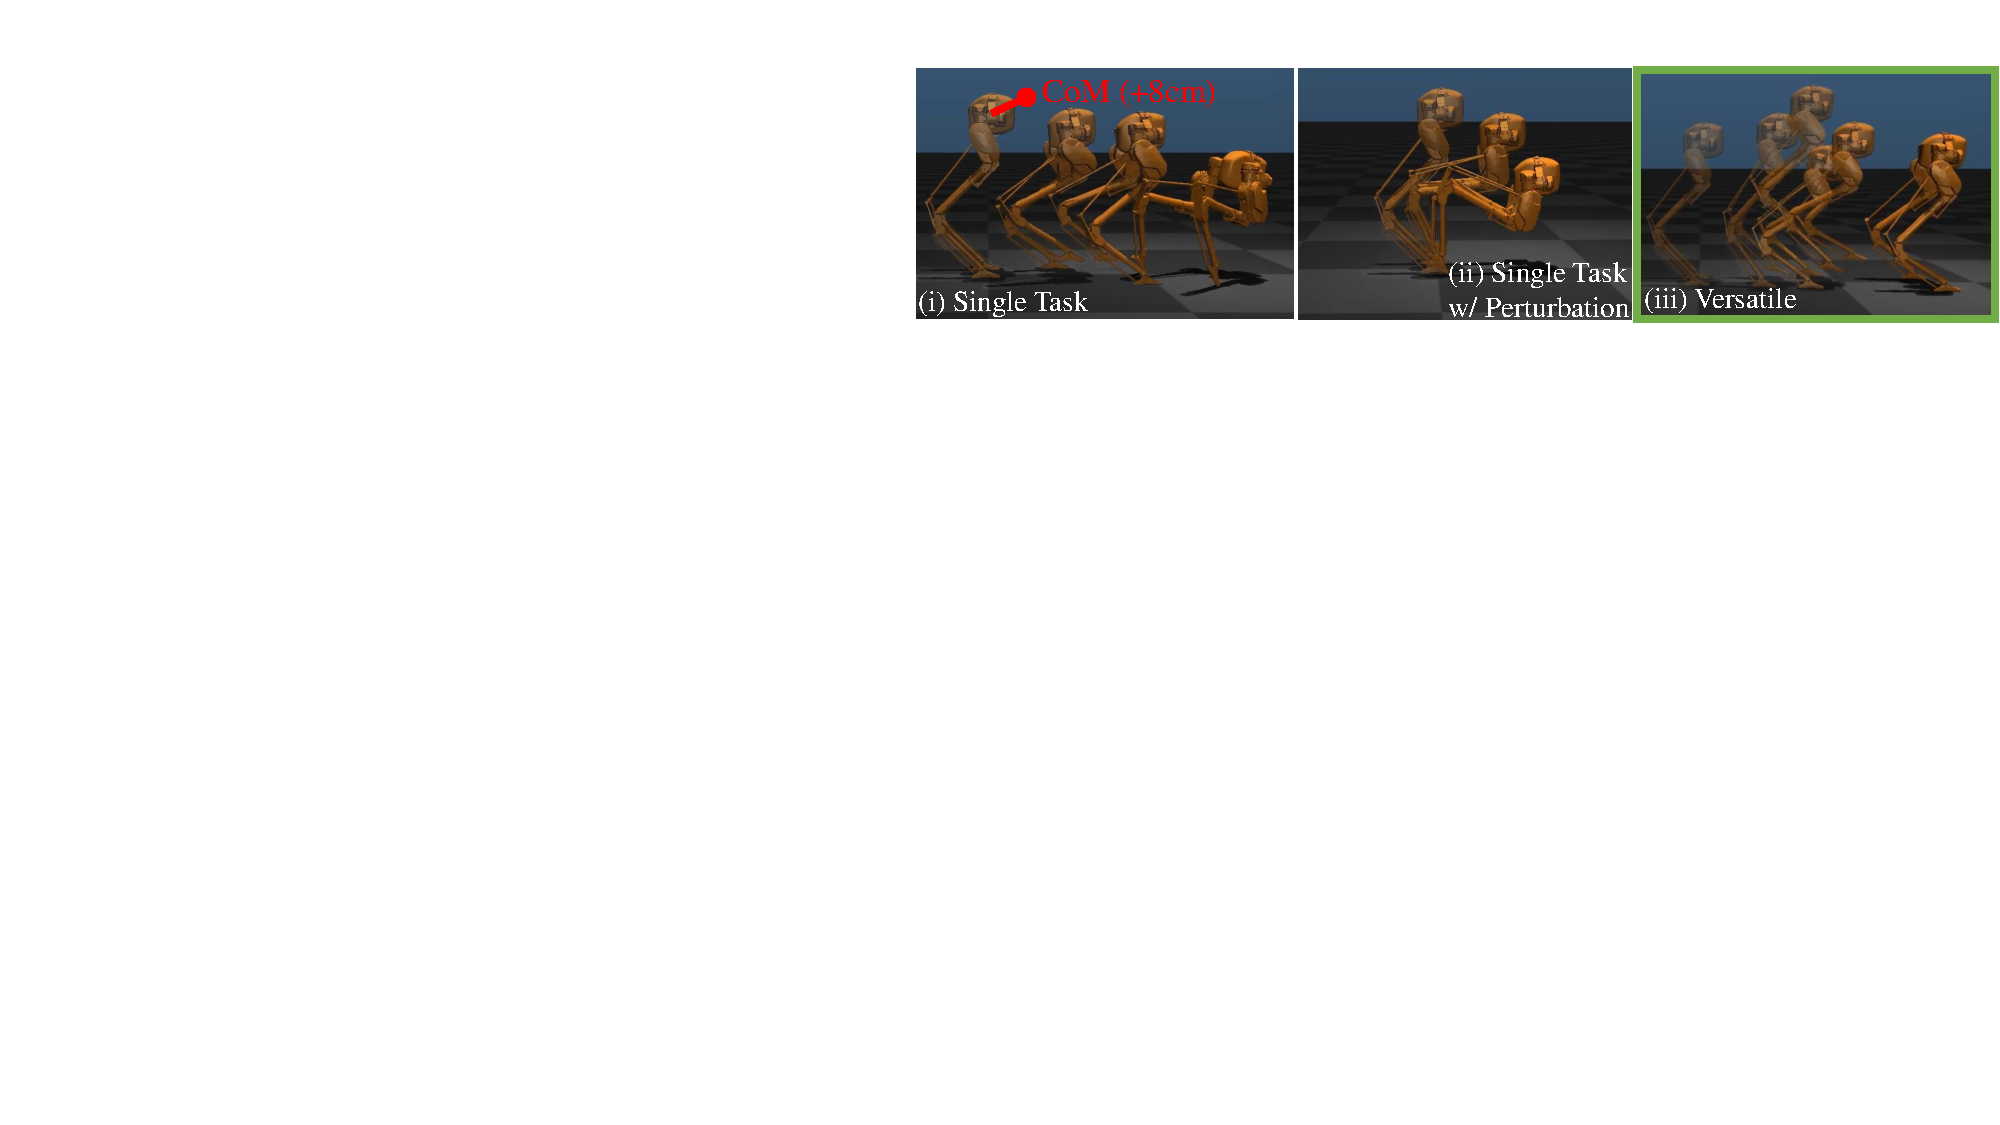
\includegraphics[width=\linewidth]{figures/bm_jump_ipos.pdf}
  \caption{Jumping with Errors in Center of Mass Positions of All Links}
  \label{subfig:bm_single_sim_ipos_jump}
\end{subfigure}

\caption{Robustness test in simulation (MuJoCo). We conduct an ablation study to evaluate the relationship between the robustness and task randomization using the baselines developed in Sec.~\ref{subsec:multi_skill_baselines}. The green bounding box indicates the scenario where the policy successfully controlled the robot without falling over. The robot is subjected to consistent perturbation forces (with its direction marked by a red arrow) or CoM position offsets of all links (with the robot's entire CoM conceptually drawn as a red point) while performing fixed locomotion tasks like walking at 0.6 m/s, running at 3 m/s, or jumping in place. Policies focused on a single task, even with extensive dynamics randomization, failed in these out-of-distribution scenarios. With additional perturbation training, the robot can maintain stability during walking, as seen in Fig.~\ref{subfig:bm_single_sim_perturb_walk}ii and Fig.~\ref{subfig:bm_single_sim_ipos_walk}ii. However, such policies are less effective for more dynamic skills like running or jumping, as illustrated in Fig.~\ref{subfig:bm_single_sim_perturb_run}ii and Fig.~\ref{subfig:bm_single_sim_ipos_jump}ii.
In contrast, a versatile policy, trained across a variety of tasks, exhibits better robustness even without specific perturbation training. The robot changes its gait under external perturbations or CoM shifts, as demonstrated by using lateral (Fig.~\ref{subfig:bm_single_sim_perturb_walk}iii) and backward walking gaits (Fig.~\ref{subfig:bm_single_sim_ipos_walk}iii), highlighting the compliance of versatile controllers. This compliance is also observed during running and jumping (Fig.~\ref{subfig:bm_single_sim_perturb_run}iii and Fig.~\ref{subfig:bm_single_sim_ipos_jump}iii), which is the key to success in these challenging robustness tests.}
\label{fig:bm_single_sim}
% \vskip-10pt
\end{figure*}




We now validate another key finding in this study, which is the source of robustness when using RL to obtain a locomotion controller, in both simulation and the real world. 
Our findings indicate that, in the context of bipedal locomotion control, a single versatile policy capable of executing various tasks can significantly improve the robustness compared to policies specialized in individual tasks. This is realized by task randomization and generalization.




\subsection{Baselines}\label{subsec:multi_skill_baselines}
We conduct a benchmark among the proposed versatile policies and task-specific baselines across all four distinct locomotion skills, including standing, walking, running, and jumping. For each of these four skills, we develop three policies, and they are:
\begin{itemize}[leftmargin=9pt]
    \small
    \item \textbf{Single Task}: The policy that is only trained with a single fixed task and dynamics randomization (excluding simulated perturbations). For walking, the task is to walk forward at 0.6 m/s; for running, the task is running at 3 m/s; for jumping, the task is to jump in place; and for standing, the task is to stand still.
    \item \textbf{Single-Task w/ Perturbation}: The policy that is trained with the same fixed task, same dynamics randomization as the \textbf{Single-Task} policy, but is also trained with additional simulated perturbations.  
    \item \textbf{Versatile (Ours)}: The policy that is trained to handle the complete spectrum of commands (tasks) detailed in Table~\ref{tab:command}, with the dynamics randomization but \emph{without} any perturbations. For the walking and running versatile policies, they also learned the transition between locomotion and standing. 
\end{itemize}



All of them used the proposed policy structure as shown in Fig.~\ref{fig:controller} and have trained with the same range of dynamics randomization introduced in Sec.~\ref{subsec:domain_rand} until convergence. For the policies trained with simulated perturbations, the range of perturbation is also the same as specified in Table.~\ref{tab:randomization}.

The above-mentioned policies are examples trained with three different methods: (1) dynamics randomization (single-task policies trained \emph{without} simulated perturbations), (2) perturbation training (single-task policies trained \emph{with} perturbations during dynamics randomization), and (3) task randomization (versatile policies). \emph{Usually, perturbation training is considered as an additional dynamics randomization.}

\subsection{Source of Robustness}
We first start our validation in a simulation, which provides a controlled and safe environment to assess the robustness of the control policies. 
In this validation, we are going to show that the robustness of a versatile locomotion policy comes from two key factors: (1) the generalization of trained randomized dynamics parameters introduced by \emph{dynamics randomization}, and (2) the generalization of various trained locomotion tasks, thereby endowing the robot with notable \emph{compliance}, brought by \emph{task randomization}.

For each locomotion control policy we've developed (including walking, running, and jumping), we test them under two distinct forms of uncertainties: (1) applying a consistent force on the robot's pelvis, and (2) introducing a significant deviation in the CoM position for all links of the robot, as depicted in Fig.~\ref{fig:bm_single_sim}. 
It's important to note that these uncertainties exceed the bound used during training, as outlined in Table~\ref{tab:randomization}. 
For example, unlike the impulse perturbation used during training, here we apply a consistent perturbation, and the CoM position offset is greater than what was covered in the training scenarios. 
The results of these out-of-distribution tests are illustrated in Fig.~\ref{fig:bm_single_sim}.


Consider the example of a walking task: when a robot is commanded to walk forward and faces a consistent lateral pulling force of 22 N, a single-task policy tailored for forward walking fails due to the lateral perturbation pushing the robot beyond its training distribution, as seen in Fig.~\ref{subfig:bm_single_sim_perturb_walk}(i). 
However, if the robot is trained with perturbation using a single-task policy, it can progress forward with minor lateral deviation under such force, shown in Fig.~\ref{subfig:bm_single_sim_perturb_walk}(ii).
In contrast, using a versatile policy that is not trained with perturbations but trained with various walking tasks, the robot still stabilizes and performs the forward walking task, albeit differently. 
This is evident from Fig.~\ref{subfig:bm_single_sim_perturb_walk}(iii), where the robot significantly deviates to the right, using learned side walking skill to compensate for the external force, resulting in a \emph{compliant} gait.

Similar results are observed with a CoM position offset of $-8$ cm in all links. Without training for perturbations or other tasks, the robot, even with randomized CoM training, cannot handle this deviation, as shown in Fig.~\ref{subfig:bm_single_sim_ipos_walk}(i). 
When trained with perturbation, since the robot has learned to stabilize under a backward force, it uses such a learned control strategy to counter the backward CoM position offset and keep walking forward with a reduced speed, as depicted in Fig.\ref{subfig:bm_single_sim_ipos_walk}(ii). 
Yet, using a versatile policy without perturbation training, the robot instead leverages backward walking gaits to offset the rearward CoM shift, as seen in Fig.~\ref{subfig:bm_single_sim_ipos_walk}(iii).




\begin{figure*}[t]
\centering
\begin{subfigure}{0.154\linewidth}
  \centering
  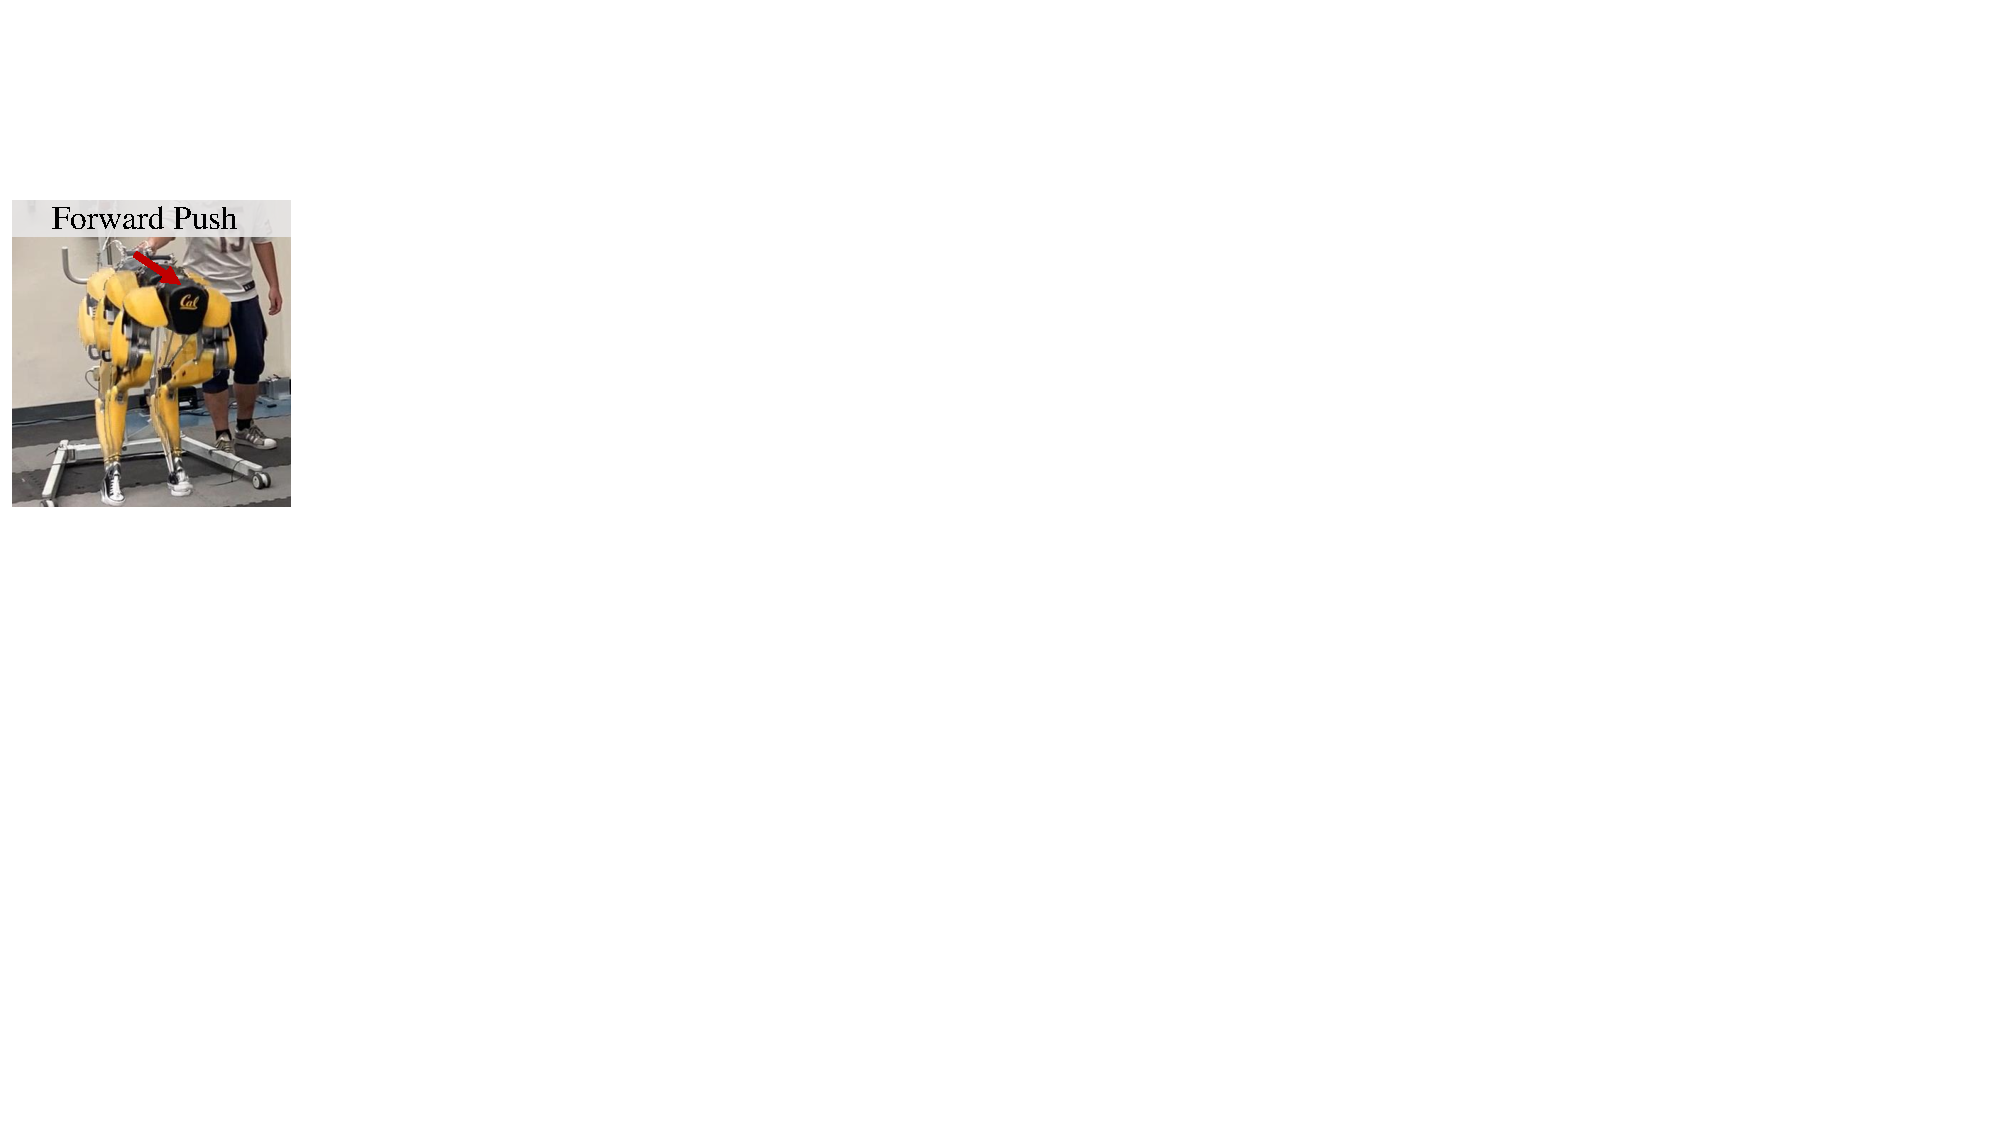
\includegraphics[width=\linewidth]{figures/bm_multi_stand_only.pdf}
  \caption{Standing skill only}
  \label{subfig:bm_multi_stand_only}
\end{subfigure}
\begin{subfigure}{0.154\linewidth}
  \centering
  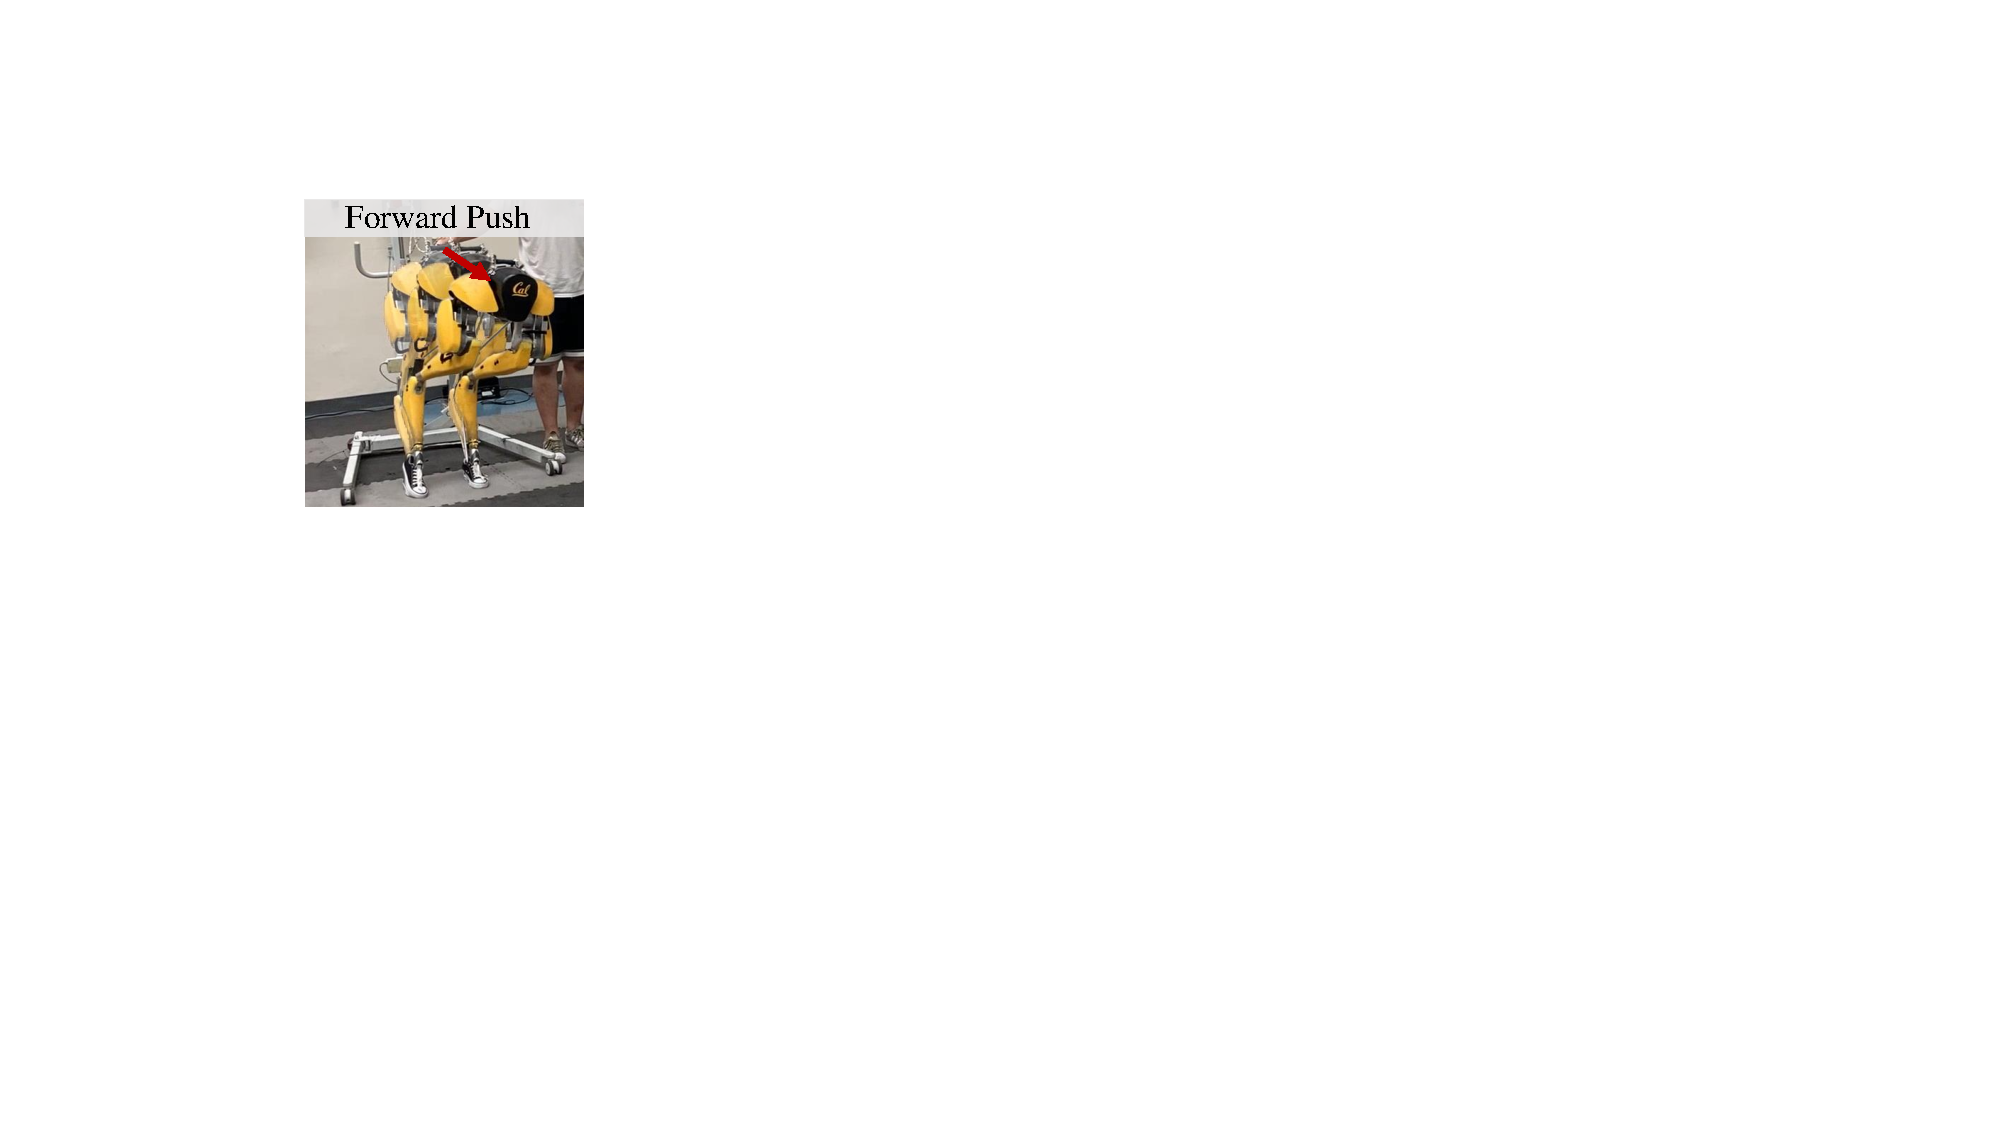
\includegraphics[width=\linewidth]{figures/bm_multi_stand_perturb.pdf}
  \caption{With perturbation}
  \label{subfig:bm_multi_stand_perturb}
\end{subfigure}
\begin{subfigure}{0.68\linewidth}
  \centering
  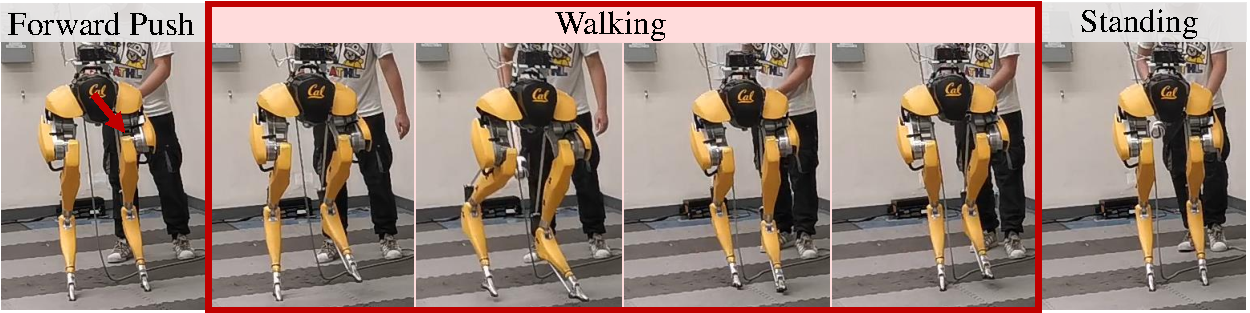
\includegraphics[width=\linewidth]{figures/bm_multi_proposed.pdf}
  \caption{Trained with both walking skill and standing skill (trained without perturbation)}
  \label{subfig:bm_multi_walking}
\end{subfigure}
\caption{Robustness test for bipedal standing skill in the real world. If the robot is trained exclusively with the standing skill, regardless of whether it underwent extensive dynamics randomization with (Fig.~\ref{subfig:bm_multi_stand_perturb}) or without simulated perturbation (Fig.~\ref{subfig:bm_multi_stand_only}), the robot tends to fall when pushed beyond its support region. In contrast, the robot using our versatile policy, trained in both walking and standing skills as shown in Fig.~\ref{subfig:bm_multi_walking}, demonstrates better robustness. Despite not being trained with perturbation during standing, the robot can spontaneously break contact when pushed forward and employ its generalized walking skills to regain its standing pose. The video of such a comparison is recorded in Vid. 3 in Table~\ref{tab:video_list}.}
\label{fig:robust_standing}
\end{figure*}


\begin{figure*}[!htp]
\centering
\begin{subfigure}{0.9\linewidth}
  \centering
  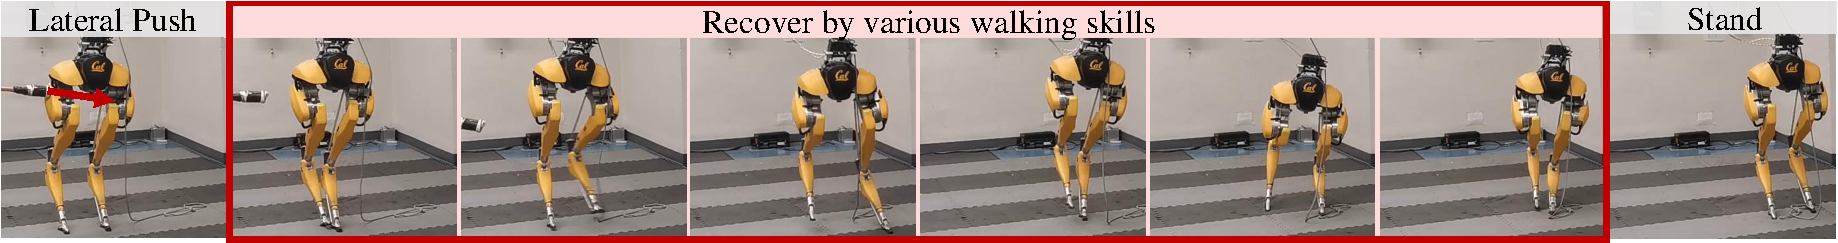
\includegraphics[width=\linewidth]{figures/stand_recover_by_walking.pdf}
  \caption{A complex recovery maneuver using various walking skills (walking sideway, backwards, and changing heights) after being perturbed during standing}
  \label{subfig:stand_recover_by_walk}
\end{subfigure}
\begin{subfigure}{0.575\linewidth}
  \centering
  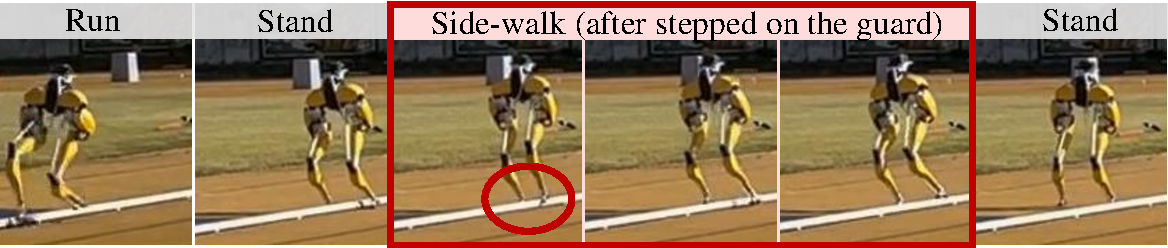
\includegraphics[width=\linewidth]{figures/stand_recover_by_running.pdf}
  \caption{Robust standing maneuver aided by running skills}
  \label{subfig:stand_recover_by_run}
\end{subfigure}
\begin{subfigure}{0.4\linewidth}
  \centering
  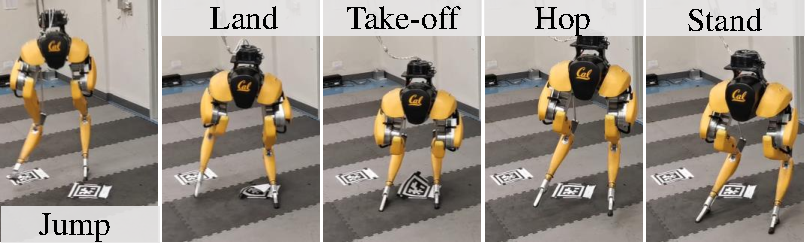
\includegraphics[width=\linewidth]{figures/stand_recover_by_jump.pdf}
  \caption{Robust standing maneuver aided by jumping skills}
  \label{subfig:stand_recover_by_jump}
\end{subfigure}
\caption{Robust bipedal standing skill realized by versatile policies in the real world. The robot, while standing, can intelligently break contact and engage learned locomotion skills as needed. For instance, as shown in Fig.~\ref{subfig:stand_recover_by_walk}, when perturbed, the robot deviates from its standing command and autonomously employs a sequence of contacts and varying walking skills over a long horizon to return to a standing position. This robustness, a result of task randomization, enhances real-world deployment capabilities. For example, in transitions to standing, like in Fig.~\ref{subfig:stand_recover_by_run}, the robot uses side-stepping skills acquired during running to aid recovery from stepping on a track guard. Similarly, with the versatile jumping skill in Fig.~\ref{subfig:stand_recover_by_jump}, the robot breaks contact after landing from an unstable state, adjusting its pose in the air for better landing, all without relying on any human-defined contact sequences.}
\label{fig:robust_standing_run_jump}
\end{figure*}




Please note that we are not trying to argue that perturbation training is inferior to task randomization. 
For example, in the walking task, robots trained with a single task and perturbations showed more favor ability to complete the assigned task (less tracking error shown in Fig.~\ref{subfig:bm_single_sim_perturb_walk}(ii), \ref{subfig:bm_single_sim_ipos_walk}(ii)), compared to those controlled by versatile policies (Fig.~\ref{subfig:bm_single_sim_perturb_walk}(iii),\ref{subfig:bm_single_sim_ipos_walk}(iii)). 
Therefore, incorporating external perturbations during dynamics randomization is still recommended following task randomization. 
However, the enhancement in robustness from simulated dynamics is not as significant as that from task randomization, especially in more dynamic tasks like running and jumping.

As depicted in Fig.~\ref{subfig:bm_single_sim_perturb_run}(i)(ii), under a constant forward perturbation of 30 N while running, policies trained only with single task fail to maintain stable gaits, regardless of extensive dynamics randomization and additional perturbation training. 
In contrast, robots using the versatile policy that has trained for faster running can adapt to such perturbations, as demonstrated in Fig.~\ref{subfig:bm_single_sim_perturb_run}(iii). 
Similar results are observed in scenarios involving a $+8$ cm CoM position offset during running (Fig.\ref{subfig:bm_single_sim_ipos_run}), and in lateral perturbation (by using a lateral jump) and forward CoM position offset (by using a forward jump) cases in jumping (Fig.~\ref{subfig:bm_single_sim_perturb_jump}, \ref{subfig:bm_single_sim_ipos_jump}). 
Note that all of these versatile policies are not trained with simulated perturbations. 

These studies highlight the two distinct sources of robustness of RL policies: (1) Training with specific simulated dynamics, including external perturbations, allows functioning within an expanded scenario range but limits the robot to the trained task; 
(2) Training with a diverse task set enables the robot to generalize learned tasks for greater robustness and compliance, even without extensive dynamics randomization.





\begin{figure}[t]
    \centering
    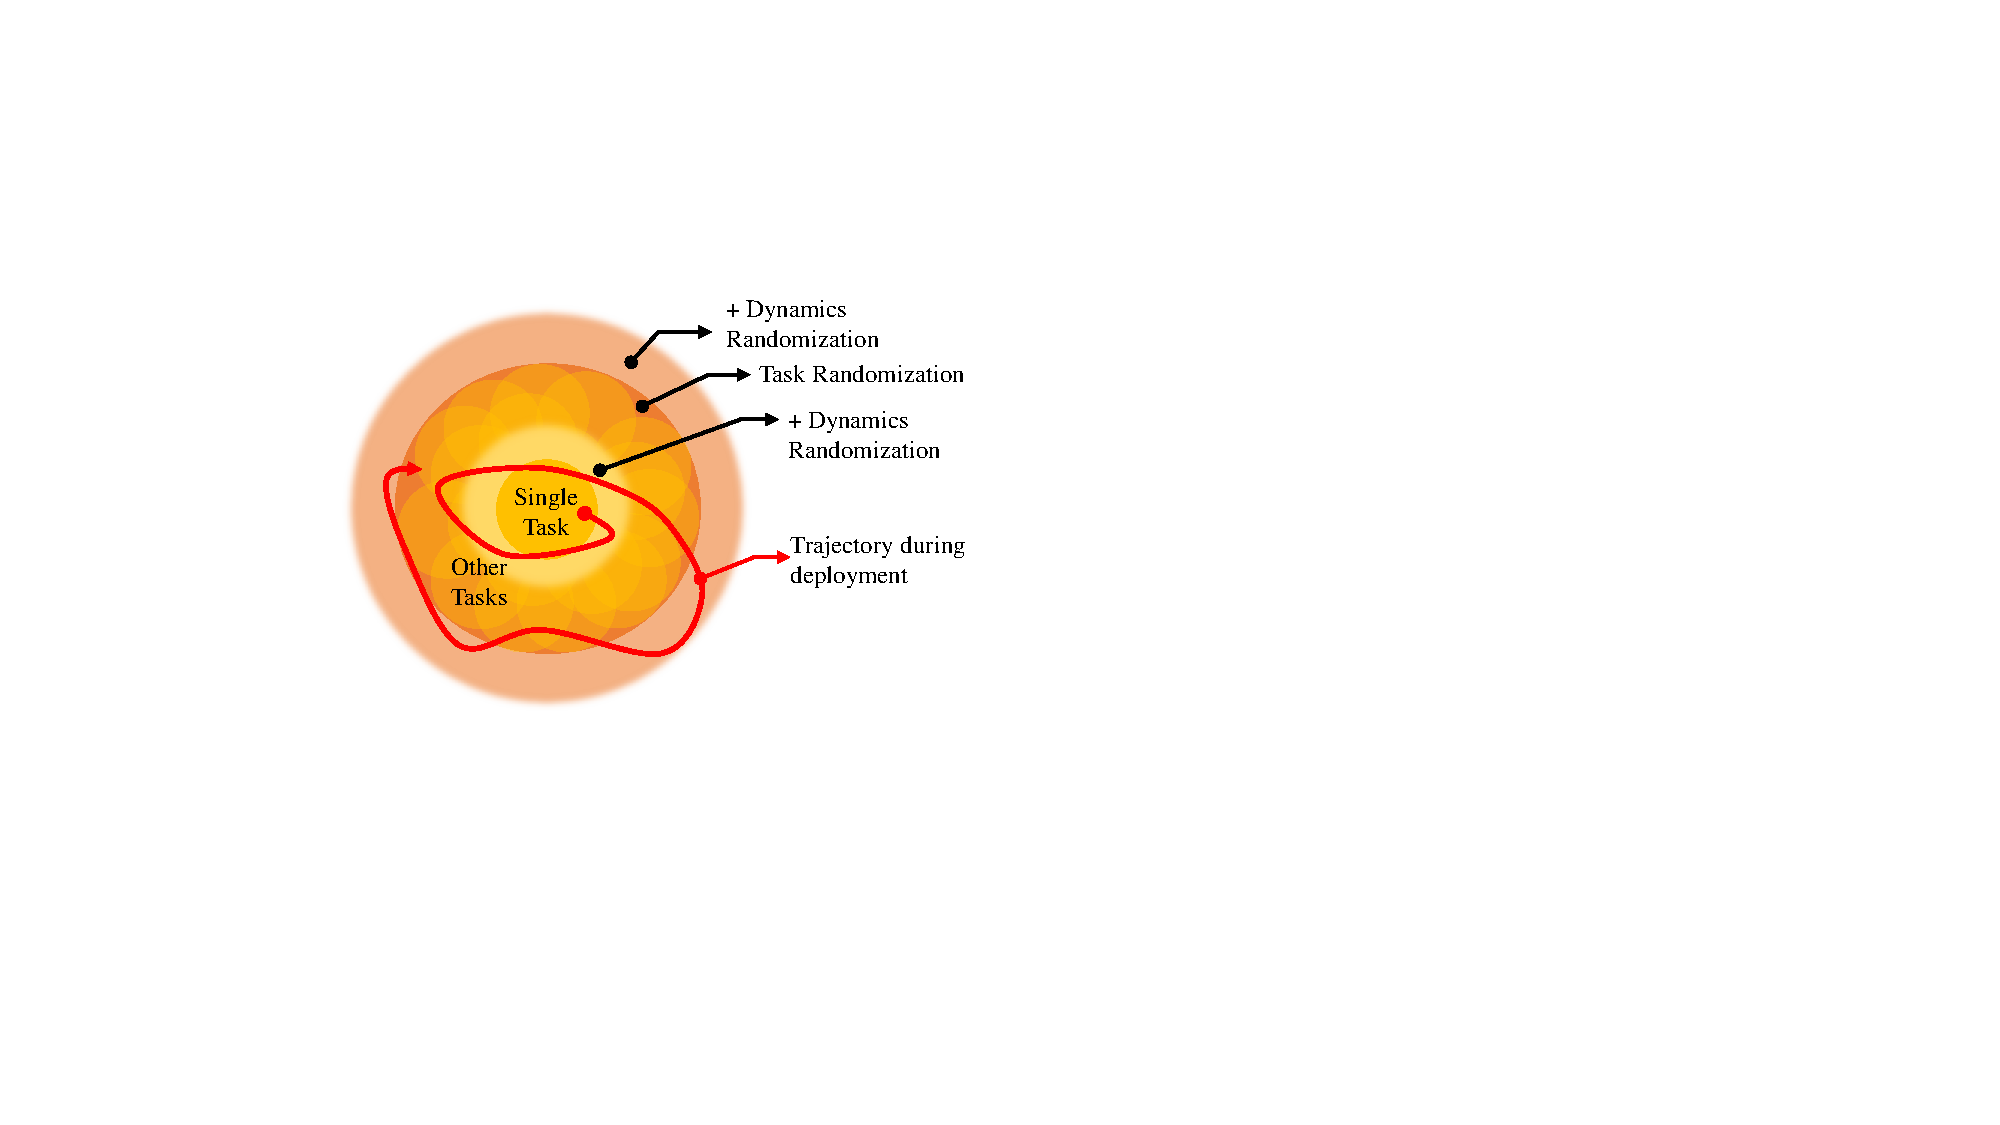
\includegraphics[width=0.7\linewidth]{figures/generalization_illustration.pdf}
    \caption{An illustration of the concept of training distributions using different methods to enhance robustness. During deployment, as conceptually illustrated by the red curve, we want the robot controlled by its RL-based policy to operate inside the training distribution of the robot's trajectories. When the training is focused on a single task, the training distribution is confined to nominal trajectories specific to that task, drawn as the yellow region. Incorporating extensive dynamics randomization, including simulated perturbations or varying terrains, can expand this distribution. However, this expansion is still centered around the fixed task. Task randomization significantly broadens the training distribution (to the orange region) by enabling the robot to learn and generalize various control strategies across different tasks (marked as different faded yellow regions). It is important to note that task randomization can be combined with dynamics randomization, further widening the training distribution and enhancing the policy's robustness.}
    \label{fig:generalization_illustration}
\end{figure}




\subsection{Case Study: Robust Standing Experiments}


We conduct a case study in the real world to gain insights into the underlying source of robustness in control policies developed through RL. 
This case study centers on evaluating the performance of the standing skill.

In this scenario, as shown in Fig.~\ref{fig:robust_standing}, we introduce an external forward perturbation to the robot's pelvis while it maintains a standing pose. 
When policies are exclusively trained for the standing skill, regardless of whether they were trained with external perturbations, the robot keeps losing its balance if it is forced to lean beyond its support region, as recorded in Figs.~\ref{subfig:bm_multi_stand_only},~\ref{subfig:bm_multi_stand_perturb}. 
Conversely, when we employ the versatile walking policy, which is also trained with the standing skill, and subject the robot to a similar forward perturbation while it is standing, as demonstrated in Fig.~\ref{subfig:bm_multi_walking}, the robot initially leans forward. However, should the robot start leaning outside its support region, it demonstrates intelligent recovery maneuvers. 
It transits to a walking gait by breaking contact, executes several steps, including forward and backward walking, and then smoothly reverts to a standing pose again. 
Remarkably, this transition occurs without any human-provided commands, as the only reference motion provided is a standing motion. 
Also, we do not simulate external perturbation during the training of the standing skill using this walking policy. 


\begin{figure*}[!htp]
    \centering
    \begin{subfigure}{\linewidth}
    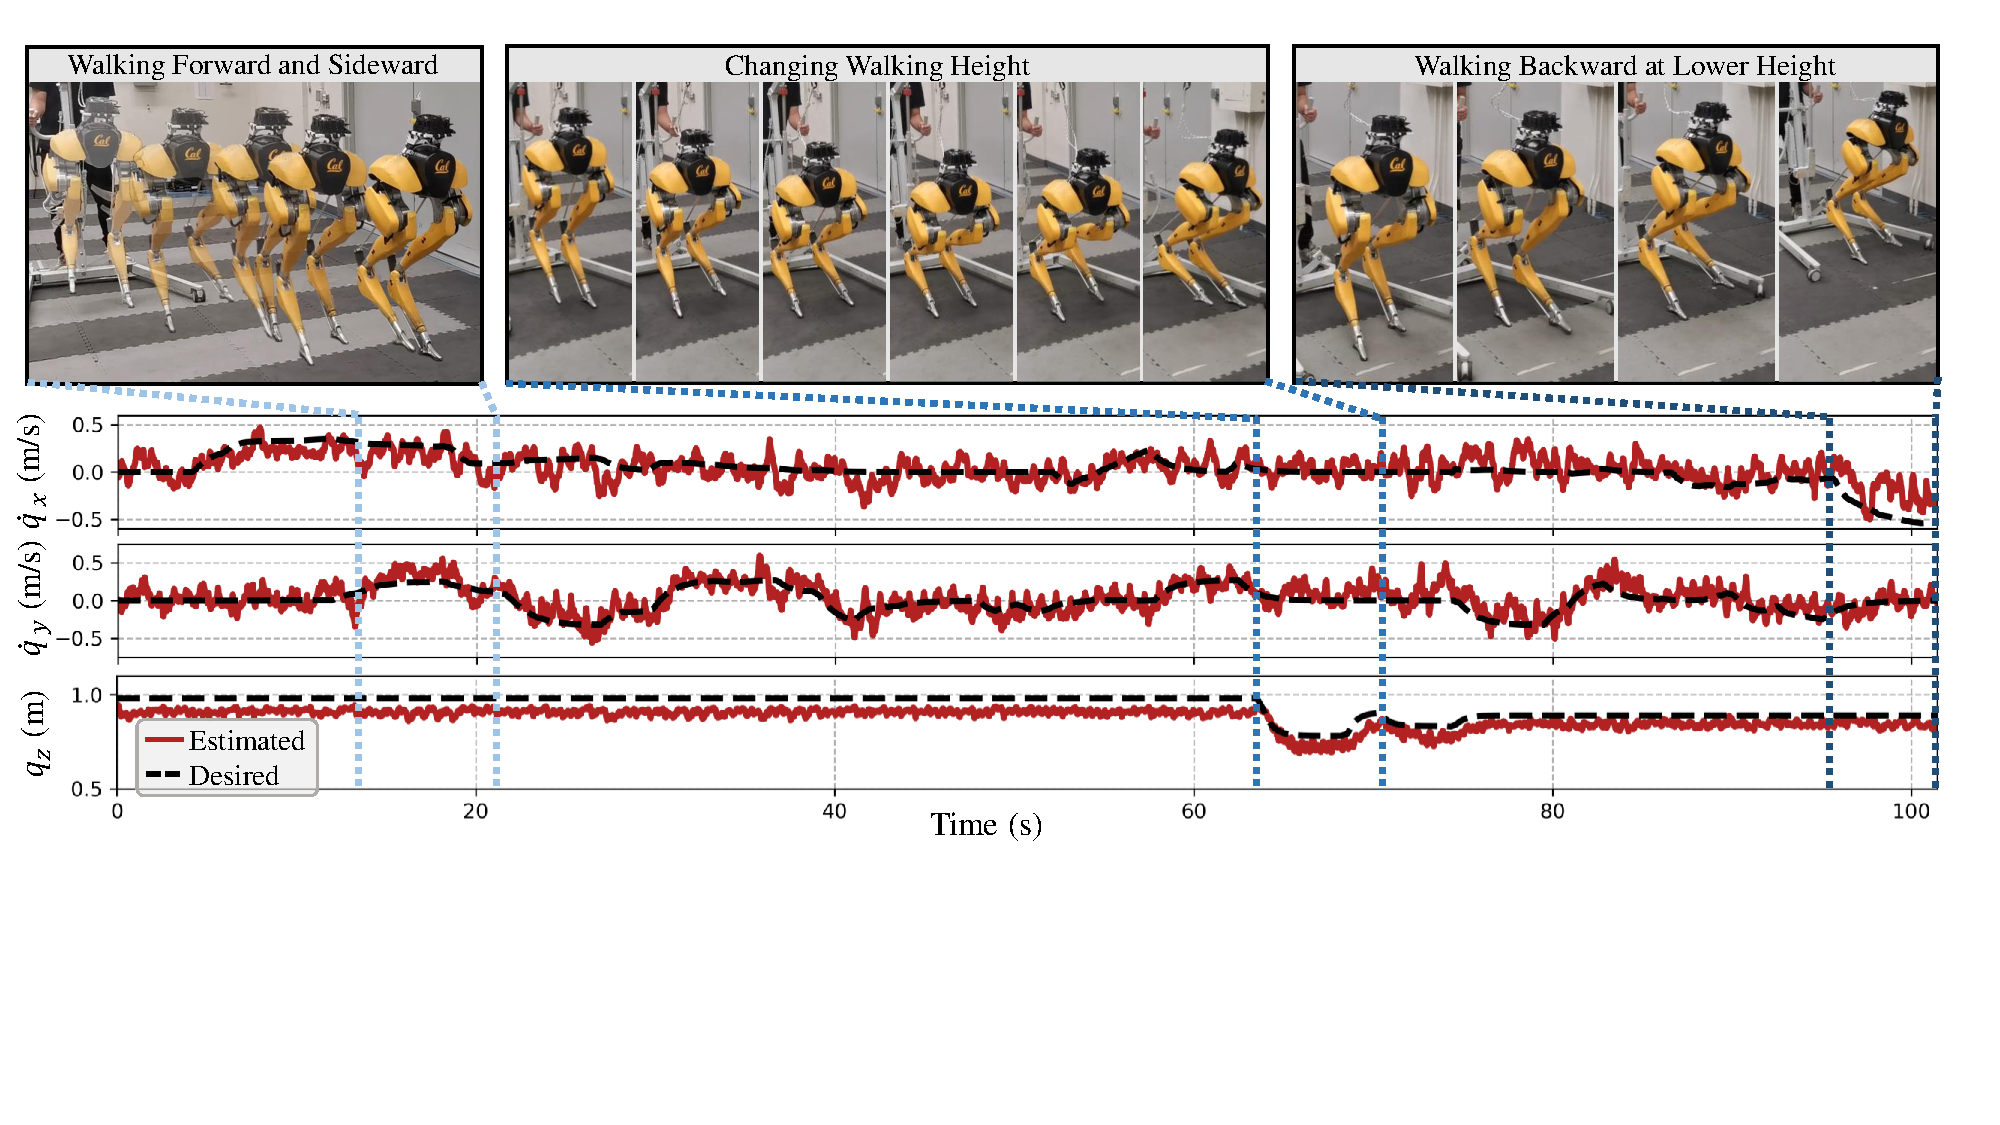
\includegraphics[width=\linewidth]{figures/variable_cmd.pdf}
    \caption{Experiments on variable command tracking conducted on August 9, 2022. The tracking errors (Mean Absolute Error, MAE) in the (sagittal velocity $\dot{q}^d_x$, lateral velocity $\dot{q}^d_y$, walking height $q^d_z$) are (0.10 m/s, 0.10 m/s, 0.06 m), respectively.}\label{subfig:variable_cmd}
    \end{subfigure}
    \begin{subfigure}{\linewidth}  
    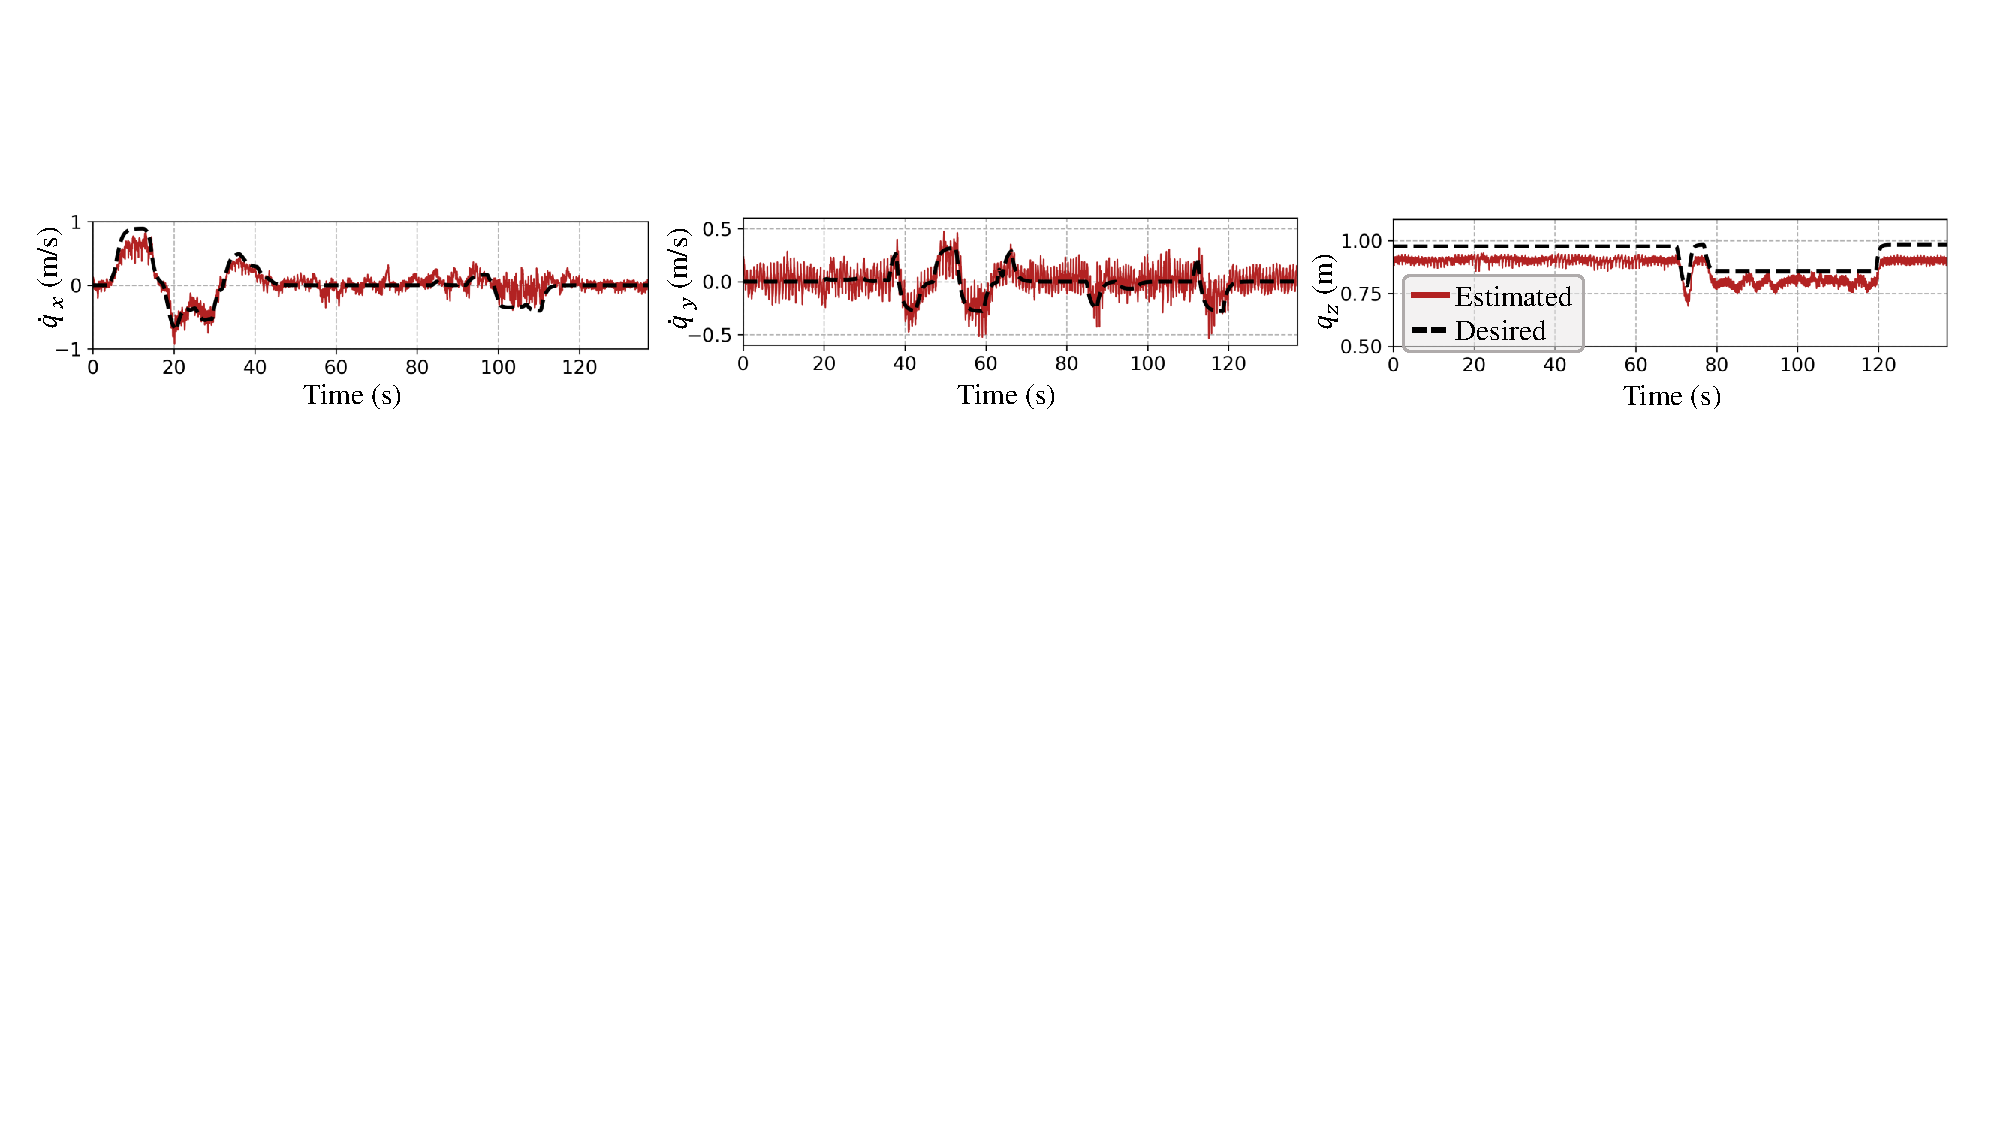
\includegraphics[width=\linewidth]{figures/variable_walking_0630.pdf}
    \caption{Experiments on variable command tracking conducted on June 30, 2023, 325 days after the one conducted Fig.~\ref{subfig:variable_cmd} using the same controller without any tuning. The tracking errors (MAE) in the $(\dot{q}^d_x, \dot{q}^d_y, q^d_z)$ directions are (0.10 m/s, 0.08 m/s, 0.06 m), repsectively}\label{subfig:variable_cmd_1214}
    \end{subfigure}
    \begin{subfigure}{\linewidth}
    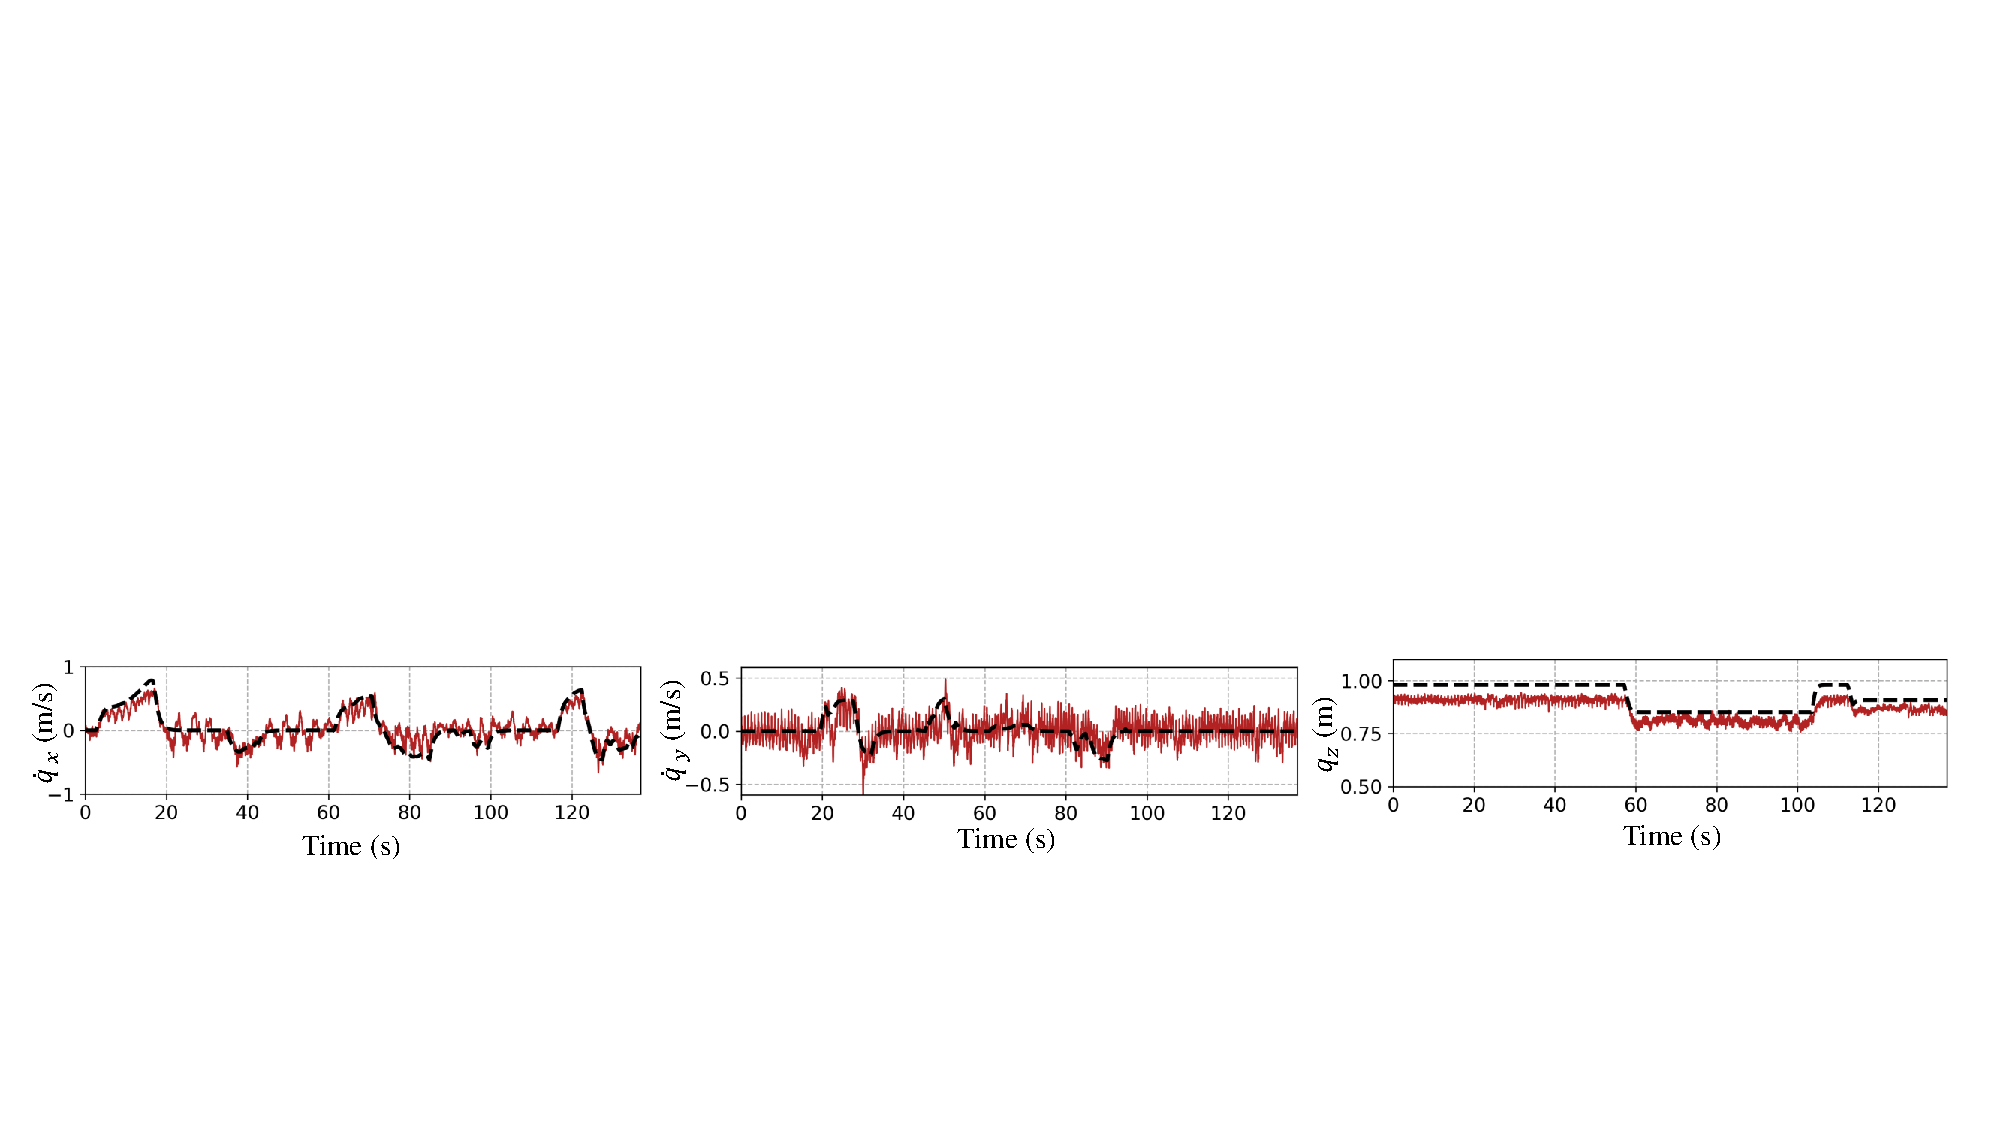
\includegraphics[width=\linewidth]{figures/variable_walking_1214.pdf}
    \caption{Experiments on variable command tracking conducted on December 14, 2023, 492 days after the one conducted in Fig.~\ref{subfig:variable_cmd} using the same controller without any tuning. The tracking errors (MAE) in the $(\dot{q}^d_x, \dot{q}^d_y, q^d_z)$ directions are (0.11 m/s, 0.09 m/s, 0.05 m), respectively}\label{subfig:variable_cmd_0630}
    \end{subfigure}  
    \caption{Fig.~\ref{subfig:variable_cmd} records a snapshot of the robot reliably tracking varying commands using the obtained versatile walking controller in the real world. The desired command and actual estimated values are recorded onboard during the experiments and drawn in the lower part. The dashed blue lines match the corresponding interval of frames in the real world. The robot can track different desired commands including changing sagittal velocity $\dot{q}^d_x$, lateral velocity $\dot{q}^d_y$, and walking height $q^d_z$, with a considerable accuracy that has a tracking error over a long test. Similar variable command tracking experiments are conducted after a long timespan, such as the one conducted after 325 days in Fig.~\ref{subfig:variable_cmd_0630} and the one after 492 days in Fig.~\ref{subfig:variable_cmd_1214}. Although the robot hardware has been changing due to wear and tear after such a long time, the same RL-based controller can still effectively control the robot to track variable commands with similar tracking errors, without any tuning in the real world.}\label{fig:variable_cmd}
\end{figure*}





The presence of a robust standing skill is highly advantageous in real-world deployments.
For example, when the robot is laterally perturbed while standing, as shown in Fig.~\ref{subfig:stand_recover_by_walk}, it utilizes its varied walking skills to recover and return to a stand. This complex sequence, transitioning through various walking maneuvers to lower its center of mass and then resuming a standing pose, highlights the policy's capability for long-horizon recovery maneuvers. 
Notably, this sophisticated recovery was not specifically trained but is a natural outcome of the versatile policy.
This benefit extends to other skills as well. 
When using the versatile running policy, as seen in Fig.~\ref{subfig:stand_recover_by_run}, the robot halts from running and steps on the track guard, as recorded in Fig.~\ref{subfig:stand_recover_by_run}.
Without loss of balance, the robot promptly disengages from the guard and uses its acquired side-stepping skills when learning the running skill, and maintains a stable stance pose afterward.
Similarly, with the versatile jumping policy (Fig.~\ref{subfig:stand_recover_by_jump}), after an unstable landing from a complex multi-axis jump, the robot executes a corrective hop, which is learned from diverse jumping tasks, to better correct itself in the air and to have a more stable landing configuration. These results can be better seen in the videos listed in Table~\ref{tab:video_list}.







\subsection{Understand Robustness from Training Distributions}
The above-mentioned findings can be conceptually illustrated in Fig.~\ref{fig:generalization_illustration}, similar to the notion of an \emph{invariant set} in control theory. 
To effectively control the robot, an RL policy needs to address a range of disturbances encountered during deployment. 
A model-free RL policy can be particularly effective when the robot's trajectory lies within its training distribution, as the policy has been specifically trained and optimized for such scenarios.
Single-task policies have a limited training distribution, focused only on that task, and training with random dynamics w/wo perturbations can extend this distribution, as shown in Fig.~\ref{fig:generalization_illustration}.
However, as evidenced in Fig.~\ref{fig:bm_single_sim}, dynamics randomization only modestly expands this distribution, primarily enhancing robustness within the single-task scheme.
In contrast, task randomization broadens the training distribution significantly. 
By enabling the robot to handle diverse tasks, this approach can effectively expand the range of the trained robot's I/O trajectory. 
When faced with disturbances during deployment, the robot can still remain within this enhanced training distribution, as illustrated in Fig.~\ref{fig:generalization_illustration}.
When combined with dynamics randomization after the task randomization, as proposed in our work in Fig.~\ref{fig:multi_stage_training}, the training distribution can further expand substantially and therefore enhance the robustness of the RL policy.






\begin{remark}
    The range of dynamics randomization can not be arbitrarily large as it will introduce significant challenges during training (the robot may fail to learn meaningful skills). The dynamics randomization range used in this work (Table.~\ref{tab:randomization}) is challenging enough for Cassie to learn, which can be evident by the low converged training return in Fig.~\ref{fig:dynrand_three}. Further adding dynamics randomization has limitations as suggested in~\cite{xie2021dynamics}. Therefore, task randomization can be viewed as an “orthogonal" way to improve the robustness rather than further pushing the range of the dynamics randomization. 
\end{remark}



\subsection{Summary of Results}
In conclusion, compared to policies focused solely on specific tasks, versatile policies exhibit significant improvements in robustness, which is validated in both simulation and the real world. 
This enhanced robustness stems from their ability to generalize learned tasks and to find better maneuvers to tackle unforeseen situations without being limited to adhering to given commands, ultimately leading to better stability. 
In RL-based locomotion control, one key source of robustness is the capacity to perform versatile tasks. 
Hence, task randomization, which diversifies the tasks during training, is recommended for future development on legged locomotion control.